% Regret, Measured: Auditing Curriculum Level Scores Against Optimal Control
% First draft (18 Oct 2026). Build:  cd paper && latexmk -pdf main.tex
%
% Conventions used throughout this draft
%   \RESULT{...}  placeholder for a number or claim that only the experiments can supply.
%                 Nothing inside a \RESULT is a finding.
%   \VERIFY{...}  a fact, citation detail or definition that is NOT stated in the repo's
%                 docs (docs/plan, docs/paper, docs/findings, docs/STATUS.md) and must be
%                 checked against the primary source before submission.
%   \TODO{...}    work that is planned but not done, or a known gap in the draft.
%   % src: PATH   every number in the text carries a comment naming the repo file it comes
%                 from (code, test or doc). Numbers without such a comment are definitions
%                 or placeholders.
%   refs.bib      bibliographic provenance lives in an unprinted `provenance` field; an
%                 entry with an open VERIFY carries \bibverify in its printed note.
% Set \draftfalse to hide the \VERIFY, \TODO and \bibverify markers. They must all be
% resolved first: \draftfalse only hides them (each remaining \bibverify then logs a
% warning), and placeholders such as the Monette et al. title in refs.bib and every
% \RESULT still print.

\documentclass[10pt]{article}

% ---------------------------------------------------------------- page and fonts
% ICLR-like single column: 5.5in x 9in text block, Times-like text and maths.
\usepackage[letterpaper,textwidth=5.5in,textheight=9in,top=1in,headheight=12pt,headsep=25pt]{geometry}
\usepackage[T1]{fontenc}
\usepackage[utf8]{inputenc}
\usepackage{amsmath}
\usepackage{newtxtext,newtxmath}
\usepackage{microtype}
\usepackage{bm}

% ---------------------------------------------------------------- tables, figures, lists
\usepackage{booktabs}
\usepackage{array}
\usepackage{tabularx}
\usepackage{longtable}
\usepackage{multirow}
\usepackage{graphicx}
\graphicspath{{../docs/findings/}}
\usepackage[font=small,labelfont=bf,skip=4pt]{caption}
\usepackage[shortlabels]{enumitem}
\setlist{itemsep=1pt,topsep=3pt,parsep=0pt}
\usepackage{siunitx}
\sisetup{group-separator={,},group-minimum-digits=4}

% ---------------------------------------------------------------- references
\usepackage[round,authoryear]{natbib}
\usepackage{xcolor}
\definecolor{linkblue}{RGB}{0,0,128}
\usepackage[colorlinks=true,linkcolor=linkblue,citecolor=linkblue,urlcolor=linkblue]{hyperref}
\usepackage[capitalise,nameinlink,noabbrev]{cleveref}
\usepackage{url}
% Function names in typewriter that may break at underscores (url.sty breaks at "_").
\DeclareUrlCommand\fn{\urlstyle{tt}}
\renewcommand{\bibfont}{\small}
\setlength{\bibsep}{2pt plus 1pt}

% ---------------------------------------------------------------- section style
\usepackage{titlesec}
\titleformat{\section}{\normalfont\large\bfseries}{\thesection}{0.8em}{\MakeUppercase}
\titleformat{\subsection}{\normalfont\normalsize\bfseries}{\thesubsection}{0.8em}{}
\titleformat{\paragraph}[runin]{\normalfont\normalsize\bfseries}{}{0pt}{}[.]
\titlespacing*{\section}{0pt}{12pt}{6pt}
\titlespacing*{\subsection}{0pt}{9pt}{4pt}
\titlespacing*{\paragraph}{0pt}{6pt}{0.6em}
\setlength{\parindent}{0pt}
\setlength{\parskip}{5.5pt}

% ---------------------------------------------------------------- draft markers
\newif\ifdraft
\drafttrue
\definecolor{resultcol}{RGB}{0,110,60}
\definecolor{verifycol}{RGB}{190,0,0}
\definecolor{todocol}{RGB}{200,100,0}
\newcommand{\RESULT}[1]{{\color{resultcol}[\textsc{result}: #1]}}
\newcommand{\VERIFY}[1]{\ifdraft{\color{verifycol}\,[\textsc{verify}: #1]}\fi}
\newcommand{\TODO}[1]{\ifdraft{\color{todocol}\,[\textsc{todo}: #1]}\fi}
% Used in refs.bib notes for entries whose fields are not yet verified.
\newcommand{\bibverify}{\ifdraft{\color{verifycol}\,[\textsc{verify}: fields, see
  refs.bib]}\else\PackageWarning{refs.bib}{An entry still carries an unresolved
  VERIFY}\fi}

% ---------------------------------------------------------------- notation
\newcommand{\Jstar}{J^{*}_{20}}
\newcommand{\Jhund}{J^{*}_{100}}
\newcommand{\Jpi}{J^{\pi}}
\newcommand{\Jhat}{\hat{J}^{\pi}}
\newcommand{\Reg}{\mathrm{Reg}}
\newcommand{\Regn}{\mathrm{Reg}_{\mathrm{norm}}}
\newcommand{\Rmax}{R_{\max}}
\newcommand{\Rgmax}{R^{\gamma}_{\max}}
\newcommand{\PLRp}{PLR\textsuperscript{$\perp$}}
\newcommand{\code}[1]{\texttt{#1}}
\newcommand{\ind}{\mathbf{1}}
\newcommand{\dev}[1]{\textsc{dev}-#1}
\newcommand{\eg}{e.g.,\ }
\newcommand{\ie}{i.e.,\ }
\DeclareMathOperator*{\argmax}{arg\,max}
\DeclareMathOperator{\std}{std}

% ---------------------------------------------------------------- title block
\title{Regret, Measured: Auditing Curriculum Level Scores\\Against Optimal Control}
\author{Anonymous authors\\Paper under double-blind review}
\date{}

\makeatletter
\renewcommand{\maketitle}{%
  \begin{flushleft}
    {\LARGE\bfseries \@title \par}
    \vspace{1.2em}
    {\normalsize \@author \par}
    \ifdraft\vspace{0.6em}{\small\color{todocol}Draft of 18 October 2026. Every
      \textsc{result} is a placeholder; every \textsc{verify} must be checked before
      submission.\par}\fi
  \end{flushleft}
  \vspace{0.8em}}
\makeatother

\begin{document}

\maketitle

% Abstract. Results are placeholders only (\RESULT); the plan's outcome table
% (docs/plan/two-track-plan.md section 2.5) lists the claims each outcome would license.
\begin{center}
  {\large\bfseries Abstract}
\end{center}
\vspace{-0.4em}
\begin{quote}
Curriculum methods for unsupervised environment design (UED) choose training levels with
scores such as positive value loss and MaxMC, which stand in for the agent's regret on
each level. Whether they rank levels by regret has so far been checked only
indirectly: against success rate at a single checkpoint, or through the downstream
performance of the curriculum. The reason is that outside gridworlds nobody knows a
level's optimal return. We build a domain where it can be computed. In a JAX racing
benchmark of
% src: src/apexzero/tracks/levels.py (SIZES: 1,000 + 300 + 100 + 4,000)
\num{5400} procedurally generated levels, a training-objective optimal control problem
(TO-OCP) solves the agent's own discounted problem on each level, with the same
integrator, 20\,Hz control rate, constraints and reward as the environment. Every
solution is checked by replaying its controls in the float64 simulator. The solver
returns a best-known rather than a certified global optimum, so the regret we measure is
a lower bound on true regret. With this answer key we audit six headline level scores
across training, on fresh rollouts and inside the buffers of real \PLRp{} and SFL runs,
and we compare curricula, including an oracle-regret arm, on one labelled pool. Fresh
scores \RESULT{rank fidelity (Spearman $\rho$, RC@10\%) per estimator and training
phase}; in-buffer fidelity \RESULT{in-buffer $\rho$ and admission AUROC, relative to
fresh fidelity}; the error is explained mainly by \RESULT{the dominant E2 term: critic
bias, dispersion, ceiling gap, success saturation or staleness}; on held-out levels the
oracle-regret curriculum \RESULT{beats / matches / loses to} PVL, MaxMC, SFL and domain
randomisation; and a replication in JaxUED's maze with its own code \RESULT{agrees /
disagrees}. The simulator, the labels and the audit harness will be released.
\end{quote}

\section{Introduction}
\label{sec:intro}

Unsupervised environment design (UED) trains a generalist by choosing which levels it
practises on. Most current methods are motivated by minimax regret: a level is worth
replaying when the gap between the best achievable return on it and the agent's return is
large~\citep{jiang2021robustplr,dennis2020paired}. That gap needs the optimal return on
every level, which is unknown in almost every domain of interest. So the methods use
proxies computed from the agent's own rollouts. Robust Prioritised Level Replay
(\PLRp{})~\citep{jiang2021robustplr}, which builds on level replay~\citep{jiang2021plr},
ranks levels by positive value loss (PVL) or by MaxMC, the gap between the best return
seen on a level and the critic's value. Newer regret proxies include maximised negative
advantage (MNA)~\citep{mead2026mna} and a transition-prediction term added to PVL in
TRACED~\citep{cho2026traced}. Other scores target something else. Sampling for
Learnability (SFL) ranks levels by $p(1-p)$, where $p$ is the success
rate~\citep{rutherford2024noregrets}; No Regrets proposes it in place of regret
approximations, as the probability of improving times the room left to improve, not as
an estimate of regret.
% src: docs/paper/sources-sfl.md section 1.1 ("justified as (probability of improving) x
%      (room left to improve)")
PACE~\citep{yuan2026pace} scores the parameter change of a provisional update, a measure
of learning progress, and the spread of a critic ensemble, an option in the minimax
library~\citep{minimax2023code}, has antecedents in curricula driven by value-ensemble
disagreement~\citep{zhang2020vds,kanitscheider2022autodime}.
% src: docs/paper/sources-recent.md sections (b2) and (d)

\paragraph{The problem} The regret proxies are treated as regret estimates, but whether
they rank levels by regret has not been checked where it matters. For the scores that
target something else, how far they agree with regret is a comparison of targets, which
is also unmeasured. The closest test, in No
Regrets~\citep{rutherford2024noregrets}, correlates PVL and MaxMC with \emph{success
rate} for one policy, one seed and one checkpoint in single-agent JaxNav, on levels
stratified by that same policy's success; it reports Pearson $r = 0.61$ for MaxMC and
$0.51$ for PVL against success,
% src: docs/paper/sources-sfl.md section 3.1 (Fig. 2a, 2b) and section 3.3
and never compares any score with regret. Exact-regret curricula exist in gridworlds,
where a shortest-path solver gives the optimum~\citep{beukman2024remidi,abdelsadek2025goal},
but they use the oracle to sample levels rather than to audit the estimators. The newer
scores are judged by the test performance of the curriculum they
drive~\citep{mead2026mna,cho2026traced,yuan2026pace}, which mixes the quality of the score
with everything else the curriculum does. In our literature search we found no paper from
2024--26 that compares UED level scores with exact or best-known regret across training.
% src: docs/plan/two-track-plan.md section 2.7 ("Verdict")
\VERIFY{re-run the search before submission: ICLR 2027 submissions and NeurIPS 2027
accepted papers, as scheduled in docs/plan/two-track-plan.md section 2.7}

The difficulty is the answer key. Regret is defined in the agent's own units, its
discounted return, so the reference has to be the optimum of that same objective, on the
same dynamics, at the same control rate and under the same termination rules. A lap-time
optimum or a success indicator measures something else. Any mismatch between the
reference problem and the agent's problem then shows up as ``regret'' that no policy
could remove.

\paragraph{Our instrument} We build a continuous-control domain in which the level-wise
optimum of the agent's own objective can be computed (\cref{sec:env,sec:answer}). A level
is an open, procedurally generated race-track strip, a car, a hidden grip value and a
start state. One vehicle model, a dynamic single-track car in curvilinear coordinates,
is written once and compiled twice: to JAX for the reinforcement-learning simulator and to
CasADi for optimal control. On $10^{4}$ random states the two agree to
% src: tests/test_dynamics.py::test_jax_casadi_parity (threshold 1e-5);
%      paper/tools/gate_values.py (measured 1.65e-14)
$2\times10^{-14}$ (\cref{tab:gates}). On each level a
\emph{training-objective OCP} (TO-OCP) maximises the agent's discounted reward over the
agent's 60\,s window. It uses the environment's RK2 integrator with ten 5\,ms substeps per
50\,ms control step, a zero-order hold at 20\,Hz, the environment's termination rules as
constraints (tightened slightly where they differ, which can only lower the optimum), and
the agent's reward as its objective. We replay the optimal controls
open-loop in the float64 simulator and accept a label only if the replayed return matches.
The solver finds local optima, so we report its value $\Jstar$ as a \emph{best-known}
optimum and the measured regret $\Jstar - \Jpi$ as a \emph{lower bound} on the true
regret (\cref{sec:answer-lb}).

\paragraph{What we measure} We ask three questions (\cref{sec:protocol}). \textbf{RQ1,
fidelity:} how well do PVL, L1 value loss, MaxMC (as implemented and in a unit-consistent
variant), MNA and ensemble disagreement rank levels by regret, on fresh rollouts and
inside the buffers that real \PLRp{} and SFL runs keep? We measure SFL's learnability
the same way, but because it targets learning potential rather than regret, its
agreement with regret is a comparison of two targets, not a test of an
estimator. \textbf{RQ2,
dynamics:} how does fidelity change with training phase, critic privilege and
observability, and which measured term explains the change? Two exact identities split
each score's error into critic bias, dispersion, the gap between the best observed and
the optimal return, success saturation and staleness (\cref{sec:est-identities}).
\textbf{RQ3, consequence:} on one labelled pool, does a \PLRp{} curriculum scored by
oracle regret beat \PLRp{} with PVL or MaxMC, SFL and domain randomisation on held-out
regret? A replication in JaxUED's maze~\citep{coward2024jaxued}, run with JaxUED's own
code and an exact breadth-first-search optimum, checks that the racing results are not an
artefact of one bespoke domain. The scorer, the window design, the level partition, the
endpoints and the decision rules are frozen in two tags, \code{audit-v1} and
\code{protocol-v1}, before any full-scale result exists (\cref{sec:prereg}).

\paragraph{Contributions}
% src: docs/plan/two-track-plan.md section 2.1 (contributions 1-4)
\begin{enumerate}
  \item A JAX racing benchmark of about \num{5400} levels, each labelled with the
        replay-verified best-known optimum of the agent's own objective.
  \item To our knowledge, the first audit of UED level scores against ground-truth (here
        best-known) regret across training, both on fresh rollouts and inside real
        curriculum buffers.
  \item A comparison of curricula on a single shared labelled pool, including an
        oracle-regret arm.
  \item A replication of the audit in JaxUED's maze, using JaxUED's own training code at
        its defaults.
\end{enumerate}
The algebraic identities we use to decompose score error (\cref{sec:est-identities}) are
a measurement framework for RQ2, not a contribution.
% src: docs/plan/two-track-plan.md section 2.1 ("The algebraic identities in E2 ...")

\paragraph{Scope} Every claim is about the racing domain and, where stated, the maze. The
racing reward is dense; whether our findings carry over to sparse-reward domains is a
conjecture we do not test (\cref{sec:threats}). No audit or curriculum experiment uses a
real circuit. Real circuits enter the paper in three ways only: twelve development
circuits supply the generator's corner statistics; the development checks of
\cref{sec:env,sec:answer} (one specialist agent, a minimum-time replay gate and the
TO-OCP spike) ran on development circuits only; and \cref{app:snapping} audits public
human telemetry, which no claim uses. No number in the paper is computed on the twelve
lockbox circuits held out for later work (\cref{sec:threats}).
% src: docs/plan/two-track-plan.md sections 2.4 ("Real circuits are left out of the paper"),
%      2.6 (reward density stated as conjecture) and 4 (lockbox rules)

\section{Related work}
\label{sec:related}
% Facts in this section come from docs/paper/sources-{jaxued,sfl,recent}.md and
% docs/plan/novelty-and-outputs.md (appendix C1, C2). Anything those files do not state is
% marked \VERIFY. Bibliographic details missing from the docs are flagged in refs.bib.

\paragraph{UED and level scores} PAIRED framed environment design as a game in which a
teacher maximises the student's regret~\citep{dennis2020paired}.\VERIFY{PAIRED's content
is not summarised in the repo docs} Robust PLR~\citep{jiang2021robustplr} replays
levels in proportion to a score and, in its \PLRp{} form, takes gradient steps only on
replayed levels. Its two scores are PVL, the time-averaged positive part of the GAE
advantage, and MaxMC, the time-averaged gap between the highest return achieved on the
level and the critic's value (\S4.2 of that paper).
% src: docs/paper/sources-jaxued.md section 1.2 ("The two papers' versions")
ACCEL~\citep{parkerholder2022accel} adds a mutation step that edits replayed levels and
scores the children with the same rule; SAMPLR~\citep{jiang2022samplr} addresses
aleatoric uncertainty in level parameters.\VERIFY{SAMPLR's content is not summarised in
the repo docs} We use the reference implementations in JaxUED~\citep{coward2024jaxued},
whose score functions are a modified copy of minimax's~\citep{minimax2023code}; the
details we replicate, and where we deviate, are in \cref{sec:estimators}. SFL, introduced
in No Regrets~\citep{rutherford2024noregrets}, scores a level by $p(1-p)$ following
\citet{tzannetos2023procurl}, keeps the top $K$ of $N$ fresh levels, and mixes uniform
draws from that set with fresh levels.
% src: docs/paper/sources-sfl.md sections 1.1 and 2.1
Its authors restrict SFL to deterministic, binary-outcome domains and suggest the
variance of rewards over repeated plays of a level as the continuous analogue.
% src: docs/paper/sources-sfl.md section 1.1 ("Scope (Sec 9)")

\paragraph{Checking scores against regret} No Regrets is the closest precedent. It
correlates MaxMC and PVL with success rate (Pearson $r = 0.61$ and $0.51$) and with mean
return, on \num{2500} JaxNav levels stratified by the success rate of the same policy
that is scored, using the final checkpoint of one PLR-MaxMC seed.
% src: docs/paper/sources-sfl.md section 3.1 (protocol; reported values table)
Its released analysis code computes no statistic between any score and regret or
learnability, and its
``Perfect Regret (Oracle)'' arm is $1-p$ on solvable levels, a success-rate proxy rather
than a return gap.
% src: docs/paper/sources-sfl.md sections 3.1 ("The statistic"), 3.2 and 3.3
ReMiDi~\citep{beukman2024remidi} runs \PLRp{} with perfect regret from a shortest-path
optimum in mazes and shows that a regret-maximising sampler can fixate on levels whose
regret cannot be reduced, which motivates its refinement of minimax regret.
% src: docs/paper/sources-recent.md ("ReMiDi"); docs/plan/novelty-and-outputs.md (C2)
\citet{abdelsadek2025goal} define oracle-latest, the exact maximum discounted return minus
the agent's latest empirical return, computed by a graph solver in gridworlds, and
compare it with a MaxMC-like max-latest score by the behaviour of the resulting agents,
not by any correlation with true regret.
% src: docs/paper/sources-recent.md section (c); docs/plan/novelty-and-outputs.md (C2)
Our oracle arm reuses their definition. \citet{monette2025} is also related.\VERIFY{the
repo docs list Monette et al.\ (RLC 2025) without any summary; read it and state the
relationship}

\paragraph{New scores judged downstream} MNA~\citep{mead2026mna} replaces the critic's
value with a running maximum over $n$-step returns, gates the score on whether the level
was ever solved, and is evaluated by zero-shot test performance on MiniGrid, Key-MiniGrid
and Sokoban.
% src: docs/paper/sources-recent.md section (a); docs/plan/novelty-and-outputs.md (C2)
TRACED~\citep{cho2026traced} adds a transition-prediction loss to PVL and a
co-learnability bonus; PACE~\citep{yuan2026pace} scores a level by the squared parameter
change of a provisional update, which measures learning progress rather than regret.
% src: docs/paper/sources-recent.md sections (b1) and (b2)
Ensemble value disagreement exists as a score option in minimax, with no published
evaluation that we found, and in goal and task curricula such as
VDS~\citep{zhang2020vds} and AutoDIME~\citep{kanitscheider2022autodime}; none of these
is a regret estimate.
% src: docs/paper/sources-recent.md section (d)
All of these are judged by what the curriculum achieves. Our audit asks the earlier
question of whether the score ranks levels by regret at all, which a downstream benchmark
cannot separate from everything else the curriculum does.

\paragraph{Learning and optimal control in racing} GT Sophy~\citep{wurman2022sophy}
and \citet{fuchs2021} trained racing policies with a two-output steering and pedal
action at 10\,Hz; Fuchs et~al.\ used soft actor-critic with a non-terminal wall-contact
penalty proportional to $\lVert v\rVert^2$, without which their cars did not learn to
brake.
% src: docs/plan/plan-v1.md section 4 (Action; Reward and episodes)
\VERIFY{GT Sophy facts and bibliographic details are not in the repo docs beyond the
action layout, the 10\,Hz rate and a speed-scaled preview of about 6\,s}
\citet{song2023reaching} compare reinforcement learning with optimal control on the same
drone model on fixed tracks, attributing RL's advantage to robustness, with no zero-shot
test.
% src: docs/plan/novelty-and-outputs.md (C1, C3 appendix)
\citet{hoeppke2022thesis} pairs PPO with direct-collocation minimum-lap-time optimisation
on one shared bicycle model: a policy trained on 8 real F1 layouts finds valid
trajectories on 18 of 20 circuits, 12 of them unseen, scored by completion or distance
rather than by a gap to the optimum, and RL is used to warm-start the collocation.
% src: docs/plan/novelty-and-outputs.md (appendix C1, Hoeppke)
\citet{green2026drone} train a zero-shot generalist drone racer with a procedural
generator and a learning-progress curriculum, and compare it with optimal control
(MPCC/MPCC++) on a single track (5.42\,s against 5.38\,s).
% src: docs/plan/novelty-and-outputs.md (appendix C1, Green et al.)
Environment as Policy~\citep{wang2025envaspolicy} learns a track-shaping teacher rewarded
by the racer's performance percentiles, and CENIE~\citep{teoh2025cenie} runs PLR with an
approximate (PVL-style) regret score plus novelty on CarRacing, the Box2D benchmark with
procedural B\'ezier tracks that Robust PLR evaluates zero-shot on 20 real F1 layouts by
return.
% src: docs/plan/novelty-and-outputs.md (appendix C1 and C2)
None of these scores a level with a time-optimal or return-optimal planner, and none
audits a curriculum score. Our use of optimal control is the reverse of most of this work:
it does not compete with the learner or train it, it grades the teacher.

\paragraph{Method precedents} Auditing estimators against ground truth across many
policies has a precedent in the DOPE benchmark for off-policy
evaluation~\citep{fu2021dope};\VERIFY{DOPE is named in the plan without a summary} we
borrow its framing for level scores. Interval estimates and aggregate statistics follow
rliable~\citep{agarwal2021rliable}.

\section{Environment and vehicle model}
\label{sec:env}
% Everything in this section is read from the code at the branch point (commit e1ac0ba):
% src/apexzero/vehicle/{params,dynamics,sim}.py, src/apexzero/env/{racing,adapters}.py,
% src/apexzero/tracks/{generator,levels,corners}.py. Gate results are from tests/ and
% docs/STATUS.md. The simulator is not yet frozen: the plan tags it as `sim-v1` before any
% audit label is computed (docs/plan/two-track-plan.md section 4, K5).

The domain is built so that the agent's problem and the optimiser's problem are the same
problem. One vehicle ODE is written against a thin operations shim and compiled twice:
to JAX for the vectorised simulator and to CasADi for optimal control. The track enters
the dynamics only through the reference curvature $\kappa(s)$, and both compilations
evaluate it, and the track widths, with the same $C^2$ cubic B-spline.
% src: src/apexzero/vehicle/dynamics.py (module docstring); src/apexzero/vehicle/sim.py

\subsection{Vehicle}
\label{sec:env-vehicle}

The car is a dynamic single-track (bicycle) model in curvilinear (Frenet) coordinates with
state $x = [s, n, \xi, v_x, v_y, r, \delta, u_p]$: arc length along the reference line,
lateral offset, heading relative to the reference, body-frame velocities, yaw rate,
road-wheel steering angle and a combined pedal state ($u_p > 0$ throttle, $u_p < 0$
brake). The policy commands $a = [a_\delta, a_p] \in [-1,1]^2$, which reach the car
through first-order actuator lags and a smooth steering-rate limit.
% src: src/apexzero/vehicle/dynamics.py (State, Input; body_derivatives)
Lateral tyre forces follow a Pacejka curve with $E = 0$ and load-sensitive friction per
tyre; each axle's longitudinal and lateral forces are scaled smoothly back onto a
friction ellipse. Downforce (split front and rear) and drag grow with $v^2$; rolling
resistance acts on the total normal load. The rear axle drives with force
$P_{\max}/v$, brakes are split by a fixed bias and fade at standstill so they cannot
reverse the car, and longitudinal load transfer uses an algebraic acceleration estimate.
Below 2--4\,m/s the model blends into a kinematic bicycle, where slip angles are
ill-conditioned.
% src: src/apexzero/vehicle/dynamics.py (tyre_forces, body_derivatives; V_BLEND_LO/HI)
Every saturation is smoothed, so the same expression is differentiable for the
optimiser. \Cref{tab:params} lists the parameters. Geometry, aerodynamics, power and
friction come from the TUMFTM lap-time simulation's F1 parameter set~\citep{tumftm_laptime},
with the mass raised to the FIA 2025 minimum; the yaw inertia, tyre shape, steering
limits, actuator lags, brake bias and brake force are our assumptions.
% src: src/apexzero/vehicle/params.py (module docstring and field comments)
\TODO{run the planned $\pm30\%$ sensitivity sweep on each assumed parameter (params.py
docstring) and report it here}

\begin{table}[t]
\centering
\small
\caption{Vehicle parameters of the default car. ``T'' marks values from the TUMFTM F1
parameter set, ``F'' the FIA 2025 minimum mass, ``A'' our assumptions. The policy
observes six context features; during training they are drawn uniformly from the ranges
in the last column, and a hidden grip multiplier $\mu_h \sim U(0.98, 1.02)$ is applied that
the policy does not observe.}
\label{tab:params}
% src: src/apexzero/vehicle/params.py (VehicleParams, CONTEXT_RANGES);
%      src/apexzero/env/adapters.py (procedural_env: mu_jitter = 0.02)
\begin{tabular}{@{}llcl@{}}
\toprule
Parameter & Value & Src. & Context range \\
\midrule
Mass $m$ & 800\,kg & F & 750--850\,kg \\
Yaw inertia $I_z$ & \num{1100}\,kg\,m$^2$ & A & -- \\
CoG to front / rear axle & 1.968 / 1.632\,m & T & -- \\
CoG height & 0.335\,m & T & -- \\
Drag area $C_dA$ & 1.56\,m$^2$ & T & 1.0--1.9\,m$^2$ \\
Downforce area $C_lA$ front / rear & 2.20 / 2.68\,m$^2$ & T & total 3.0--6.0\,m$^2$ \\
Aero balance (front share of $C_lA$) & 0.451 & T & $\pm 0.05$ \\
Air density & 1.18\,kg/m$^3$ & T & -- \\
Peak power $P_{\max}$ & 695\,kW & T & 550--800\,kW \\
Rolling resistance coefficient & 0.03 & T & -- \\
Friction $\mu_x/\mu_y$, front & 1.65 / 1.85 at 3\,kN & T & global scale 0.85--1.10 \\
Friction $\mu_x/\mu_y$, rear & 1.95 / 2.15 at 3\,kN & T & (same scale) \\
Friction load sensitivity & $-5\times10^{-5}$\,N$^{-1}$ & T & -- \\
Pacejka $B$, $C$ & 12, 1.6 & A & -- \\
Steering lock, rate limit, lag & 0.45\,rad, 1.5\,rad/s, 0.05\,s & A & -- \\
Pedal lag & 0.05\,s & A & -- \\
Brake bias (front), max.\ brake force & 0.58, 60\,kN & A & -- \\
Slip limit $\alpha_{\max}$ & 10$^\circ$ & A & -- \\
\bottomrule
\end{tabular}
\end{table}

\paragraph{Integration} The simulator integrates with the explicit midpoint rule (RK2)
at 5\,ms, ten substeps per 50\,ms control step, holding the action constant over the
control step (20\,Hz zero-order hold).
% src: src/apexzero/vehicle/sim.py (rk2_step, control_step); src/apexzero/env/racing.py (EnvParams)
The optimiser uses exactly this map (\cref{sec:answer}).

\subsection{Tracks and levels}
\label{sec:env-levels}

\paragraph{Generator} A track is an open strip of 8\,km on a 2\,m grid (\num{4096}
points), generated on the device in JAX.
% src: src/apexzero/tracks/generator.py (N_POINTS = 4096, DS = 2.0)
Each strip opens with a straight of 500--900\,m, followed by alternating corners and
straights. Corners are drawn jointly (turning angle, minimum radius, length) from the
corners of the twelve development circuits, with log-normal jitter ($\sigma = 0.15$); each
is a trapezoidal curvature profile with clothoid ramps of at least 10\,m and a radius
floor of 8\,m. The turning direction alternates with a probability that depends on the
preceding gap, which reproduces chicanes and esses. Widths come from the development
circuits' median widths with low-frequency variation, a left/right asymmetry and a cap
$(w_{\text{in}} - 1)\,\kappa \le 0.6$ on the inside of each corner, which keeps the
Frenet frame non-singular wherever the car can reach.
% src: src/apexzero/tracks/generator.py (module docstring, fit_grammar defaults, generate)
Because the simulator is local in Frenet coordinates, strips need no closure or
self-intersection checks. The development circuits are twelve real layouts from the
TUMFTM database~\citep{tumftm_tracks}. They supply these statistics, and they hosted the
development checks reported in \cref{sec:env-mdp,sec:env-gates,sec:answer-evidence}
(a specialist agent, a minimum-time replay gate and the TO-OCP spike); no audit or
curriculum experiment runs on them. A disjoint set of twelve lockbox circuits is held
out of the paper: no number reported here is computed on them (\cref{sec:threats}
discloses the one design decision a lockbox circuit influenced).
% src: src/apexzero/tracks/corners.py (R_DEV, R_TEST); tests/test_generator.py::test_dev_and_lockbox_are_disjoint
Generated corners match the development circuits' corner statistics: the
Wasserstein-1 distance for minimum radius, divided by the median radius, is 0.07.
% src: docs/STATUS.md (K5 row: "radius W1/median 0.07"); gate < 0.3 for radius, angle and
%      corner length in tests/test_generator.py::test_corner_statistics_match_development_circuits
Two variants share the support of the training generator or deliberately leave it. The
\emph{tilted} generator re-weights corners by $1/r_{\min}$ and shortens gaps by 20\%
(hairpin-heavy, still inside the training support); the \emph{out-of-distribution}
generator re-weights by $r_{\min}^{-1.5}$, lowers the radius floor to 6\,m, scales widths
by 0.65 and lengthens gaps by 60\%.
% src: src/apexzero/tracks/generator.py (tilted, out_of_distribution)

\paragraph{Levels} A level is $\theta = (g, c, \mu_h, x_0)$: a strip $g$, a car context
$c$ (the six features of \cref{tab:params}), a hidden grip draw $\mu_h$, and a start state
$x_0$. Every component is fixed per level. Every audit level starts on the opening
straight with $s = 0$, $n = 0$, $\xi = 0$, $v_x = 0.8\,v_{\text{QSS}}(0)$ and previous
action zero, where $v_{\text{QSS}}$ is the speed profile of a quasi-steady-state
point-mass oracle.
% src: src/apexzero/tracks/levels.py (module docstring, START_SPEED_FRACTION, build)
A straight start keeps the heavily weighted first seconds of the discounted return from
depending on an arbitrary mid-corner state. Level sets come from disjoint, named seed
streams, so no training draw can coincide with an audit or pool level
(\cref{tab:levelsets}).
% src: tests/test_levels.py::test_level_streams_are_disjoint_and_deterministic

\begin{table}[t]
\centering
\small
\caption{Level sets. All are drawn from disjoint seed streams of the same level
constructor and frozen in \code{audit-v1}. A\textsubscript{DR}, A\textsubscript{tail} and
A\textsubscript{OOD} are both the audit sets for E1 and the held-out evaluation sets for
the curriculum comparison~C.}
\label{tab:levelsets}
% src: src/apexzero/tracks/levels.py (STREAMS, SIZES); docs/plan/two-track-plan.md section 2.4
\begin{tabular}{@{}lrll@{}}
\toprule
Set & Levels & Generator & Role \\
\midrule
A\textsubscript{DR} & \num{1000} & training & i.i.d.\ audit set; phases defined on it \\
A\textsubscript{tail} & 300 & tilted & hairpin-heavy, inside the training support \\
A\textsubscript{OOD} & 100 & out-of-distribution & narrower, tighter, longer straights \\
Pool & \num{4000} & training & the only levels curricula in C may train on \\
\midrule
Total & \num{5400} & & every level labelled with $\Jstar$ \\
\bottomrule
\end{tabular}
\end{table}

\subsection{Observations, actions, reward and termination}
\label{sec:env-mdp}

\paragraph{Observation} The actor sees 222 numbers and nothing that identifies the track
or the position along it. A preview of 40 points lies ahead along the reference at
distances $d_k = d_{\max}(k/40)^{1.5}$ with $d_{\max} = \mathrm{clip}(6\,\mathrm{s}
\cdot v, 150, 500)$\,m; each point gives the left and right edge in the body frame and
the curvature (200 numbers). Sixteen ego features (velocities, yaw rate, sideslip,
position in the corridor, heading error, steering, pedal, accelerations, previous action,
friction-ellipse use and slip angles per axle) and the six normalised context features
complete it. Audit rollouts add 1\% Gaussian noise to the normalised observation.
% src: src/apexzero/env/racing.py (module docstring, observe, preview_offsets);
%      src/apexzero/audit/rollouts.py (module docstring: "1% observation noise")
\TODO{the plan's asymmetric critic (actor inputs plus track geometry every 10\,m out to
1.5\,km and the true grip; docs/plan/plan-v1.md section 4) is not implemented yet: the
current critic sees the actor's observation. E0 needs it and E0-sym needs the current
symmetric critic}

\paragraph{Action and reward} The action is $[a_\delta, a_p] \in [-1,1]^2$ at 20\,Hz.
The per-step reward is
\begin{equation}
  r_t = \frac{s_{t+1} - s_t}{10\,\text{m}} - 0.02\,\lVert a_t - a_{t-1}\rVert^2,
  \label{eq:reward}
\end{equation}
and a terminating step additionally pays $-(5 + 5\,(v/50\,\text{m/s})^2)$. Progress
$s_{t+1} - s_t$ is measured along the reference line, so the reward contains no
racing-line term; the speed-scaled crash penalty follows the observation of
\citet{fuchs2021} that fixed penalties were either ignored or made the car stop.
% src: src/apexzero/env/racing.py (step_no_reset); docs/plan/plan-v1.md section 4 (Reward)

\paragraph{Termination and truncation} An episode terminates when the car's reference
point comes within 1\,m of either track edge, when $|\xi| > 90^\circ$, when either axle's
slip angle exceeds $\alpha_{\max} = 10^\circ$ (loss of control), when the car stays below
2\,m/s for 2\,s, or on a non-finite state. It is truncated at the end of the 60\,s window
(\num{1200} control steps) or 520\,m before the end of the strip.
% src: src/apexzero/env/racing.py (EnvParams, step_no_reset)
The slip limit closes an exploit found in an early minimum-time optimum, which drifted
through a chicane far beyond the rear tyre's peak slip, on the soft post-peak part of the
tyre curve. That optimum was computed on a lockbox circuit, before the simulator was
frozen (\cref{sec:threats}). The same $10^\circ$ limit is a termination in the
environment and a constraint in every optimal control problem.
% src: docs/STATUS.md ("Things found along the way", first item: the circuit is a lockbox
%      circuit in src/apexzero/tracks/corners.py R_TEST; its slip angle and lap-time gain are
%      deliberately not reported); params.py alpha_max

\paragraph{Discount and agent} The agent optimises the discounted return with
$\gamma = 0.995$ (a 10\,s effective horizon at 20\,Hz) using PPO with GAE
$\lambda = 0.95$, written from scratch in JAX~\citep{schulman2017ppo,schulman2016gae}.
% src: src/apexzero/agents/ppo.py (PPOConfig)
Our implementation matches or beats rejax~\citep{rejax} with identical hyperparameters
and seeds (CartPole-v1: $475.3 \pm 31.9$ against $327.8 \pm 103.7$; Pendulum-v1:
$-158.5 \pm 5.9$ against $-159.5 \pm 8.3$, mean over seeds with 95\% intervals).
% src: docs/findings/ppo-verification.md
On one development circuit (Hockenheim), a single-track specialist trained for
200\,M steps completes every evaluation lap and is 4.8\% slower than the minimum-time
optimum, inside the 8\% gate the plan sets before any audit run; this is one seed of three.
% src: docs/STATUS.md (K4 row); docs/plan/two-track-plan.md section 5.2 (K4 gate)
For domain randomisation, a device-resident bank of \num{4096} strips is refreshed 256
strips at a time before every PPO update; each reset draws a strip, a car context and a
hidden grip value, and starts at a uniformly random position with a random lateral offset,
a small heading error and 60--100\% of the reference speed.
% src: src/apexzero/env/adapters.py (procedural_env defaults); src/apexzero/env/racing.py (reset)
Five extra value heads read a stop-gradient copy of the critic trunk, each trained on its
own GAE target, so the disagreement score cannot change the critic it is audited
against.
% src: docs/STATUS.md (K5 row: "critic ensemble heads with per-head targets");
%      docs/paper/score-spec.md section 1.7; scripts/train_dr.py (--ensemble-heads 5)
\TODO{freeze the E0 network and PPO hyperparameters (8,192 environments $\times$ 64
steps per the plan) in \code{sim-v1} and list them in an appendix table; the 64-step
rollout conflicts with the scorer's 128-step chunks (\cref{sec:est-notation})}

\subsection{Physics gates}
\label{sec:env-gates}

A regret label is only as good as the agreement between the simulator and the problem the
optimiser solves, and both are only useful if the car behaves like a racing car.
\Cref{tab:gates} lists the gates the model passes; each is a unit test in the repository.

\begin{table}[t]
\centering
\small
\caption{Physics and consistency gates. ``Criterion'' is the assertion in the named test.
``Measured'' is the measured value: from \code{paper/tools/gate\_values.py}, which repeats
the test's computation and prints the quantity it asserts on, from the project status
log, or from the recomputation described for the last row; ``pass'' marks tests whose
measured value we have not extracted.}
\label{tab:gates}
\begin{tabularx}{\linewidth}{@{}>{\raggedright\arraybackslash}p{2.6cm}>{\raggedright\arraybackslash}X>{\raggedright\arraybackslash}p{2.6cm}@{}}
\toprule
Gate & Criterion (test) & Measured \\
\midrule
% src: tests/test_dynamics.py::test_jax_casadi_parity (threshold and normalisation);
%      measured: paper/tools/gate_values.py (1.65e-14 normalised, 2.84e-14 absolute)
JAX--CasADi parity & largest difference of $\dot x$ over $10^4$ random states, including
the kinematic blend, divided by $\max(|\dot x|, 1)$ (relative above 1, absolute below),
$< 10^{-5}$ & $2\times10^{-14}$ \\
% src: tests/test_tracks.py::test_spline_lookup_is_identical_in_jax_numpy_and_casadi;
%      measured: paper/tools/gate_values.py (4.44e-16)
Track lookup & spline values of JAX and NumPy within $10^{-12}$ of CasADi's & $4\times10^{-16}$ \\
% src: tests/test_dynamics.py::test_terminal_speed; docs/STATUS.md (K1)
Terminal speed & analytic value 85--92\,m/s; simulated speed after 90\,s at full throttle
within 0.5\% of it & 315\,km/h \\
% src: tests/test_dynamics.py::test_coast_down_matches_1d_ode
Coast-down & speed over 20\,s from 80\,m/s within 0.05\,m/s of the 1-D drag and rolling
ODE & pass \\
% src: tests/test_dynamics.py::test_low_speed_is_kinematic
Low-speed kinematics & yaw rate within 2\% of $v_x\tan\delta/L$ at 1.5\,m/s & pass \\
% src: tests/test_dynamics.py::test_braking_deceleration_is_f1_like;
%      measured: paper/tools/gate_values.py (6.38 g, 2.50 g)
Braking & full-pedal deceleration 4--7\,g at 83\,m/s and 1.8--3.5\,g at 30\,m/s &
6.4\,g and 2.5\,g \\
% src: tests/test_dynamics.py::test_braking_to_a_stop_never_reverses
Standstill & braking to a stop never reverses the car & pass \\
% src: tests/test_dynamics.py::test_dt_convergence_open_loop; docs/STATUS.md (K1)
Integrator & RK2 at 5\,ms against RK4 at 1\,ms over 20\,s of open-loop inputs above
1\,g: distance within $5\times10^{-4}$ relative, $v_x$ within 0.02\,m/s, $n$ within
0.05\,m & distance within $3\times10^{-6}$ \\
% src: tests/test_skidpad.py; docs/STATUS.md (K1)
Skidpad & steady-state limit on $R = 30, 50, 80$\,m within 80--102\% of the point-mass
envelope, grip-limited; on $R = 400$\,m power-limited near top speed & 91--93\% of the
envelope; power-limited above $\approx$290\,km/h \\
% src: tests/test_window_ocp.py (on Hockenheim, a development circuit);
%      measured: paper/tools/gate_values.py (state 4.86e-17, lookup 2.12e-17)
TO-OCP step & CasADi step map and windowed spline equal the simulator's to $10^{-10}$
(state) and $10^{-12}$ (lookup) & $5\times10^{-17}$ (state), $2\times10^{-17}$ (lookup) \\
% src: tests/test_ocp.py::test_ocp_is_consistent_with_the_simulator (oval);
%      development circuits: recomputed on corners.R_DEV only, with the code of main at
%      355d331, by `uv run python scripts/solve_all_ocp.py --workers 3 --out
%      outputs/paper-draft/ocp-rdev --tracks <the 12 R_DEV names>`; outputs/paper-draft/
%      ocp-rdev/summary.csv: 12/12 Solve_Succeeded, |shooting_rel_err| max 1.64e-4
%      (YasMarina), median 7.0e-5. No lockbox circuit was solved for this row.
Minimum-time OCP replay & replayed lap time within $10^{-3}$ relative and position within
0.2\,m of the $s$-domain optimum on a test oval; the same replay on the 12 development
circuits & oval: pass; development circuits: 12/12 converge, lap time within
$1.6\times10^{-4}$ (median $7\times10^{-5}$) \\
\bottomrule
\end{tabularx}
\end{table}

The gates caught real defects before any learning run: the smoothed ReLU leaked throttle
and brake at neutral pedal (found by the coast-down gate), brakes kept pushing after a
stop and reversed the car, and the quasi-steady-state speed cap was a placeholder that
started open strips above top speed. Each fix has a test.
% src: docs/STATUS.md ("Things found along the way")
The last gate of \cref{tab:gates} was recomputed on the twelve development circuits
alone; no lockbox circuit was solved for it (\cref{sec:threats}).
\TODO{record the R-dev replay-gate run (command and summary in the src comment of
\cref{tab:gates}) in docs/STATUS.md, in place of the all-circuit K2a figure}

\section{The answer key: a training-objective OCP}
\label{sec:answer}
% Code: src/apexzero/ocp/window.py (TO-OCP, window mode); src/apexzero/ocp/replay.py and
% scripts/spike_to_ocp.py (replay check). Plan: docs/plan/two-track-plan.md sections 1, 2.2.
% Evidence: docs/findings/to-ocp-spike.md, docs/STATUS.md (K2a row).

\subsection{Problem}
\label{sec:answer-problem}

For a level $\theta$ with start state $x_0$ and window length $T = 1200$ control steps,
the training-objective OCP is
\begin{equation}
\begin{aligned}
  \Jstar(\theta) \;=\; \max_{a_0,\dots,a_{T-1}} \quad
    & \sum_{t=0}^{T-1} \gamma^{t}\Big[\frac{s_{t+1}-s_t}{10\,\text{m}}
      - 0.02\,\lVert a_t - a_{t-1}\rVert^2\Big] \\
  \text{s.t.}\quad
    & x_{t+1} = \Phi_\theta(x_t, a_t), \qquad a_t \in [-1,1]^2, \qquad a_{-1} = 0, \\
    & -\big(w_r(s_{t+1}) - 1\,\text{m} - \epsilon\big) \le n_{t+1}
      \le w_l(s_{t+1}) - 1\,\text{m} - \epsilon, \\
    & |\alpha_f(x_{t+1})|,\ |\alpha_r(x_{t+1})| \le \alpha_{\max}, \qquad
      |\xi_{t+1}| \le \pi/2, \qquad v_{x,t+1} \ge 2\,\text{m/s},
\end{aligned}
\label{eq:toocp}
\end{equation}
for $t = 0, \dots, T-1$, with $\gamma = 0.995$.
% src: src/apexzero/ocp/window.py (module docstring; WindowSpec: steps 1200, gamma 0.995,
%      edge_margin 1.0, safety 0.03; WindowSolver bounds)
Here $\Phi_\theta$ is the simulator's own control-step map: RK2 with ten 5\,ms substeps
and the action held for 50\,ms, the same vehicle ODE, and the level's six-feature car
context as a parameter. The solver has no separate grip input, so the hidden grip must
be folded into the context: the solver receives the context with its global friction
scale multiplied by $\mu_h$, which is how the environment builds its parameters from
$(c, \mu_h)$.
% src: src/apexzero/ocp/window.py (_context_params: ctx[0..5] only; WindowSolver.solve ctx);
%      src/apexzero/env/racing.py (params_from_context: ctx[4] * hidden_mu)
% src: src/apexzero/ocp/window.py (WindowSolver.solve(hidden_mu=): ctx_drive[4] *= hidden_mu)
\TODO{add a test that the solver's step map with folded grip equals the environment's step
for $\mu_h \ne 1$}
The constraints are the environment's non-termination set (\cref{sec:env-mdp}), applied
at every post-step state and tightened in three ways that can only lower the optimum.
First, a safety margin $\epsilon = 3$\,cm keeps a float64 replay of a solution that rides
a constraint from terminating. Second, the environment terminates only after the car has
stayed below 2\,m/s for 2\,s, while the OCP requires $v_x \ge 2$\,m/s at every step.
Third, the solver bounds $v_x \le 120$\,m/s, $|v_y| \le 25$\,m/s and $|r| \le 5$\,rad/s.
The objective is the environment's reward \eqref{eq:reward}; the crash penalty does not
appear because terminating trajectories are infeasible.
% src: src/apexzero/ocp/window.py (WindowSolver.solve: lbX/ubX, v_x lower bound 2.0);
%      src/apexzero/env/racing.py (step_no_reset: slow-for-2-s termination)
\TODO{log whether the stall bound and the auxiliary state bounds are ever active in the
label runs}

\paragraph{Exact track lookup} CasADi's B-spline node exists only for its MX graph type,
which made exact Hessians about 50 times slower. Instead, each control step $t$ carries a
window of $K$ spline coefficients around its warm-start position $\sigma_t$, and
$\kappa(s)$ and $w(s)$ are evaluated as the exact B-spline sum over that window.
Inside the window this equals the simulator's spline; $s_t$ is bounded to within 15\,m of
$\sigma_t$, and an outer loop re-centres the windows and re-solves if a solution reaches
the bound. Track coefficients, car context and $x_0$ are solver parameters, so one
compiled solver serves every level with the same window length.
% src: src/apexzero/ocp/window.py (module docstring; WindowSpec.radius = 15.0; solve loop)
The CasADi step map and windowed lookup agree with the JAX simulator to
$5\times10^{-17}$ in the state and $2\times10^{-17}$ in the lookup on a development
circuit (the test asserts $10^{-10}$ and $10^{-12}$).
% src: tests/test_window_ocp.py; paper/tools/gate_values.py (Hockenheim)
The NLP is a multiple-shooting problem with every state and action as a decision
variable ($8(T+1) + 2T$ of them) and one defect constraint per control step, solved by
IPOPT with the MUMPS linear solver~\citep{wachter2006ipopt,andersson2019casadi}.
% src: src/apexzero/ocp/window.py (WindowSolver.__init__)

\paragraph{Warm starts and labels} Every level gets the same three starts: the $s$-domain
minimum-time optimum mapped to time, the quasi-steady-state line, and the best rollout of
the final checkpoint. The label is the best value over the starts whose replay passes the
check below. The budget is uniform because a second pass only on suspicious levels would
bias where labelling effort goes.
% src: docs/plan/two-track-plan.md sections 2.2 ("Every level gets the same 3-start
%      budget") and 9 (scope critic: uniform agent-warm-start pass)

\paragraph{Replay verification} The optimal controls are applied open-loop, one action per
50\,ms, in the float64 JAX environment with its termination checks. A label is accepted
only if the replay survives the whole window and its discounted return matches the
solver's value to within 0.05\%.
% src: docs/plan/two-track-plan.md section 2.2 ("Replay in float64 must match within
%      0.05%, with a 2-5 cm margin inside the corridor"); docs/findings/to-ocp-spike.md
This closes the loop between the two compilations: if the CasADi model and the simulator
disagreed anywhere along the trajectory, the replay would drift or terminate.

\subsection{Why this is the right answer key}
\label{sec:answer-why}

UED's minimax-regret objective refers to $\max_{\pi'} J^{\pi'}(\theta) - \Jpi(\theta)$
with $J$ the agent's own expected discounted return. \Cref{eq:toocp} is that maximum for
the agent's problem, with four properties that a generic reference (a lap-time optimum,
a success indicator, a point-mass model) lacks.
\begin{enumerate}
  \item \textbf{Same objective.} Regret comes out in the agent's units, discounted
        return, which is the quantity the level scores are meant to track. A time-based
        reference is not in those units: turning a lap-time or distance gap into a return
        gap needs a conversion that depends on where in the window the time is lost, and
        that conversion would set the scale of every regret we report. The discount
        weighting the agent sees is the one the optimum sees. In one dimension
        (\cref{app:braking}) the two optima brake at the same point, to within one control
        step, at the agent's $\gamma = 0.995$ and diverge only at horizons of a few tenths
        of a second; the appendix is mainly an independent check that a discounted optimum
        built from the environment's reward and crash penalty behaves as expected.
  \item \textbf{Same discretisation and control rate.} The optimiser cannot exploit a finer
        integrator or a faster controller than the agent has, so integration error and
        the cost of acting at 20\,Hz do not appear as regret.
  \item \textbf{Same actuators, and constraints that are never looser.} The steering and
        pedal lags, the rate limit, the corridor and the slip limit are all inside
        $\Phi_\theta$ or the constraints, so the optimum is reachable by a policy acting
        through the same actuators. Where the constraints differ from the environment's
        termination rules (the margin, the stall bound, the auxiliary bounds) they are
        stricter.
  \item \textbf{Determinism per level.} Given $\theta$, the dynamics are deterministic
        (the hidden grip is fixed per level), so the best open-loop control sequence from
        $x_0$ achieves the optimal value over all policies, closed-loop or not. Optimising
        over open-loop sequences loses nothing.
\end{enumerate}
The fourth point also says what $\Jstar$ is \emph{not}: it is the optimum for an agent that
knows $\theta$. Our agent sees a 150--500\,m preview, noisy observations and a car
context, but not the hidden grip. The part of regret caused by what the policy cannot
observe is irreducible for this policy class. That is regret in the sense UED uses it,
but it is exactly the kind a regret-maximising sampler can fixate
on~\citep{beukman2024remidi}; we return to it in \cref{sec:threats}.

\subsection{A lower bound, not an estimate}
\label{sec:answer-lb}

Let $J^{\mathrm{opt}}(\theta)$ be the supremum of the window return over all control
sequences, including those that terminate. Three things can make the label fall short of
it: IPOPT returns a local optimum; the feasible set is tightened by the safety margin, the
stall bound and the auxiliary state bounds; and terminating trajectories are excluded,
although with
$\gamma^{1200} \approx 0.0024$ a late crash can in principle cost less than the progress it
buys.
% src: gamma^1200 ~ 0.0024 as stated in docs/paper/sources-jaxued.md section 4 item 3
Nothing can make it exceed $J^{\mathrm{opt}}$ if the label is the \emph{replayed} return,
because a replay is a trajectory the simulator actually produced; the solver's own value
agrees with it to within the 0.05\% acceptance tolerance.
\TODO{fix in \code{audit-v1} that the stored label is the float64 replayed return, not the
solver's objective value}
Hence $\Jstar \le J^{\mathrm{opt}}$, and for every policy
\begin{equation}
  \Reg(\theta) \;:=\; \Jstar(\theta) - \Jpi(\theta) \;\le\;
  J^{\mathrm{opt}}(\theta) - \Jpi(\theta).
  \label{eq:lowerbound}
\end{equation}
We therefore call $\Jstar$ the \emph{best-known optimum} and $\Reg$ a \emph{lower bound}
on regret throughout. Any return the agent itself realises is also a lower bound on
$J^{\mathrm{opt}}$ (up to the rounding of the single-precision rollouts), because a
realised action sequence is a feasible open-loop control; the best observed agent return
is thus a free check on the label. We report how often it
exceeds the label: \RESULT{fraction of levels, per phase, on which an observed agent
return beats $\Jstar$, and by how much}. The bound holds for the expectation $\Jpi$; a
Monte Carlo estimate $\Jhat$ can still put individual levels below zero.

Two references bracket the label from other sides. A control-rate reference $\Jhund$
solves the same window at a 100\,Hz zero-order hold, warm-started from the 20\,Hz
solution, on 200 levels; $\Jhund - \Jstar$ is the price of acting at 20\,Hz, which no
20\,Hz policy can recover. An undiscounted ($\gamma = 1$) maximum-distance variant on 600
A\textsubscript{DR} levels gives distance lost in 60\,s without discount weighting.
% src: docs/plan/two-track-plan.md section 2.2 ("Bounds and references", "Secondary targets")
Label noise is measured directly: 200 pilot levels get at least three extra starts, which
gives a per-level label standard deviation (\cref{sec:protocol-targets}).

\paragraph{The window objective and the agent's training objective} PPO bootstraps the
value at the window end, so the agent is trained for the infinite-horizon discounted
return, while \cref{eq:toocp} stops at $T$. The omitted tail is $\gamma^{T}V(x_T)$, with
$\gamma^{1200} \approx 0.0024$. The same finite horizon lets the OCP spend the last
seconds of a window in ways a time-unaware policy cannot (for example by not slowing for a
corner just beyond the window end); that gain is discounted by roughly the same factor.
We expect both effects to be small and quantify them in \cref{sec:threats}.

\subsection{Evidence so far}
\label{sec:answer-evidence}

The spike solved the TO-OCP on a 10\,s window of a development circuit (Hockenheim),
warm-started from the $s$-domain minimum-time optimum mapped to time. IPOPT converged
(\code{Solve\_Succeeded}) in 169 iterations over 3 re-centring rounds, in 44\,s of solve
time and 0.7\,GB of peak memory in a single process on a 12-thread laptop CPU. The
float64 replay reproduced the
optimum exactly ($J^* = 48.089$ both ways) and survived the window.
% src: docs/findings/to-ocp-spike.md (table)
Two very different warm starts reached the same optimum.
% src: docs/STATUS.md (K2a row)
These are one window of one circuit, a sixth of the label window length. Whether the
solver converges as reliably, and how long it takes, on 60\,s windows of procedural
strips decides the size of the label budget.
On eight production-like generated levels (8\,km strips, each with its own random car and
hidden grip), a 60\,s window, the level's own $s$-domain optimum included, took 131--520
CPU-seconds (median 206) on seven; the eighth hit IPOPT's iteration limit after 791
CPU-seconds with no verified optimum. Windows of Hockenheim took 106--189 CPU-seconds, and
every verified optimum replayed to its $J^*$ within $3\times10^{-12}$.
% src: docs/findings/to-ocp-spike.md (production-like levels pool:0-7; Hockenheim windows);
%      the benchmark's other circuit windows lie on lockbox circuits and are sealed
\RESULT{convergence rate and per-solve CPU time over the production label set}
The plan budgets 1,200--3,000 CPU-hours for about \num{5400} levels with three starts
each. Three starts sharing one $s$-domain optimum cost about 775 CPU-seconds per level at
these figures, about \num{1160} CPU-hours for \num{5400} levels; above 12 CPU-minutes per
solve the pool would shrink to \num{2000} levels and the curriculum buffer to 500.
% src: docs/plan/two-track-plan.md sections 5.2 (Spike gate) and 8 (CPU item)

\section{Level scores and how we compute them}
\label{sec:estimators}
% Everything in this section is condensed from docs/paper/score-spec.md (`audit-v1` scorer
% spec, draft for sign-off, 18 Oct 2026) and implemented in src/apexzero/audit/estimators.py.
% Section numbers "spec §x" refer to that file.

An audit of a score is only meaningful if the score is the one practitioners run. We
therefore port every score from pinned reference code, keep its behaviour wherever our
setting allows, and list every departure. The references are JaxUED at commit
\code{0f8f128} for PVL, MaxMC and the \PLRp{} buffer, minimax at \code{2ae9e04} for L1 value
loss and ensemble disagreement, the MNA authors' repository at \code{12340c7}, and the SFL
authors' repository at \code{8b14e2e}~\citep{coward2024jaxued,minimax2023code,mna2026code,sfl2024code}.
% src: docs/paper/score-spec.md section 0.1 (pinned sources)

\subsection{Notation and the scoring advantage}
\label{sec:est-notation}

One episode $e$ is one window, running over steps $t_0(e), \dots, t_{\text{end}}(e)$ with
$T_e$ steps including the terminal transition, as in JaxUED. $r_t$ is the raw reward of
\cref{eq:reward}. Our PPO trains its critic on rewards divided by a running return
standard deviation $\sigma$, so we rescale every value to raw units, $V_t := \sigma \hat
V_t$, and likewise the five ensemble heads $V^k_t$ (\dev{6}). $\mathrm{term}_t$ marks a
crash and $\mathrm{trunc}_t$ the window end. $V^f_t$ is the value of the pre-reset final
observation at a truncation, and $\kappa_t = 1$ marks the last step of a 128-step training
chunk that does not end the episode. In the fresh audit, window starts are given a random
phase $\varphi_e \sim U\{0, \dots, 127\}$ against chunk boundaries, as they have in
training. We write $G_e = \sum_{t \in e} r_t$, $G^\gamma_e = \sum_{\tau=0}^{T_e-1}
\gamma^\tau r_{t_0+\tau}$ (no bootstrap) and $\bar V_e = T_e^{-1}\sum_{t\in e} V_t$.
% src: docs/paper/score-spec.md section 0.2

The reference codebases score levels with the PPO's own GAE tensor. Ours is in scaled
units and bootstraps truncations, so we run a separate scoring pass in raw units
(\dev{6}):
\begin{equation}
  \mathrm{nxt}_t =
  \begin{cases}
    0 & \text{if } \mathrm{term}_t,\\
    0 \ \text{(mode F) or}\ V^f_t \ \text{(mode B)} & \text{if } \mathrm{trunc}_t,\\
    V_{t+1} & \text{otherwise},
  \end{cases}
  \qquad
  \begin{aligned}
  \delta_t &= r_t + \gamma\,\mathrm{nxt}_t - V_t,\\
  A_t &= \delta_t + \gamma\lambda\,(1-d_t)(1-\kappa_t)\,A_{t+1},
  \end{aligned}
  \label{eq:gae}
\end{equation}
with $d_t = \mathrm{term}_t \lor \mathrm{trunc}_t$, $\gamma = 0.995$ and the PPO's
$\lambda = 0.95$. At a chunk end ($\kappa_t = 1$) the $\lambda$-sum restarts and $V_{t+1}$,
computed with the parameters that produced $V_t$, bootstraps it.
% src: docs/paper/score-spec.md section 0.3; src/apexzero/audit/estimators.py (scoring_gae)
Mode F treats the window end as terminal, as JaxUED, minimax and the MNA code all do with
their time limits; it is the headline. Mode B bootstraps, as our PPO does, and is stored
as a variant.

\paragraph{An expected artefact of mode F} The critic has no time-in-window input, so at
every window end $\delta \approx r - V$, roughly $-60$ in raw units at racing speed. This
pushes $A_t$ strongly negative over the last $1/(1-\gamma\lambda) \approx 18$ steps, adds
about $|V_{\text{end}}| \cdot 18 / T_e$ to L1, and biases the mean advantage negative, so
$\mathrm{PVL}/\mathrm{L1} < 0.5$ even with an accurate critic. The prediction that this
ratio tends to $0.5$ as critic error shrinks can therefore only hold in mode B. We log
both modes and the tail term, the summed $|A_t|$ over the last 64 steps of each completed
window.
% src: docs/paper/score-spec.md section 0.3 ("Notes on mode F") and section 6 ("E2 wording")

\subsection{The six headline estimators}
\label{sec:est-six}

\Cref{tab:estimators} gives each score as we compute it per level from a set $\mathcal E$
of $E$ completed windows. Scores are episode-weighted means, as in the reference
accumulator. We store every score for $\lambda \in \{0.9, 0.95, 0.98, 1\}$, in mode B, and
in a discount-weighted form $\sum_\tau \gamma^\tau m_\tau / \sum_\tau \gamma^\tau$; the
appendix variants are $1-p$, return variance and step-normalised absolute learning
progress.
% src: docs/paper/score-spec.md sections 1.1-1.8; docs/plan/two-track-plan.md section 2.2
%      ("Six headline estimators", "Stored variants")
\TODO{the three appendix variants are named in the plan but not yet specified or
implemented}

\begin{table}[t]
\centering
\small
\caption{The six headline scores (seven rows: MaxMC has two variants). ``Reference'' is
the pinned function we port. All are larger for levels the score deems more worth
replaying.}
\label{tab:estimators}
% src: docs/paper/score-spec.md sections 1.1-1.7; src/apexzero/audit/estimators.py (level_scores)
\renewcommand{\arraystretch}{1.25}
\begin{tabularx}{\linewidth}{@{}>{\raggedright\arraybackslash}p{2.2cm}>{\raggedright\arraybackslash}X>{\raggedright\arraybackslash}p{2.9cm}@{}}
\toprule
Score & Per-level value & Reference \\
\midrule
L1 value loss & $\frac{1}{E}\sum_e \frac{1}{T_e}\sum_{t\in e} |A_t|$ &
  minimax \fn{compute_l1_value_loss} \\
PVL & $\frac{1}{E}\sum_e \frac{1}{T_e}\sum_{t\in e} \max(A_t, 0)$ &
  JaxUED \fn{positive_value_loss} \\
MaxMC (as implemented) & $\Rmax - \frac{1}{E}\sum_e \bar V_e$, \ $\Rmax = \max\!\big(0,
  \max_e G_e\big)$: undiscounted and floored at zero &
  JaxUED \fn{max_mc}, \fn{compute_max_returns} \\
MaxMC (unit-consistent) & $\frac{1}{E}\sum_e \big(\Rgmax - V_{t_0(e)}\big)$, \
  $\Rgmax = \max_e G^\gamma_e$: discounted, no floor, no time average & ours (\dev{22}) \\
Learnability & $\hat p(1-\hat p)$, $\hat p$ the mean of a per-window success indicator:
  S1 = the window completes; S2 = S1 and distance $\ge 0.97\,d_{\text{QSS}}(\theta)$ &
  SFL \fn{_calc_outcomes_by_agent} \\
MNA & $\hat C \cdot \sum_e\sum_{t\in e}\hat G_t \,/\, \sum_e T_e$ with the closed-form
  clipped advantage $\hat G$ below; $\hat C = \ind[\text{any window satisfied S1}]$ &
  MNA \fn{compute_clipped_gae}, \fn{negative_value_loss_solved_sum} \\
Disagreement & $\frac{1}{E}\sum_e\frac{1}{T_e}\sum_{t\in e}\std_k V^k_t$ over the five
  heads (population std; main critic excluded) & minimax
  \fn{compute_value_disagreement} \\
\bottomrule
\end{tabularx}
\end{table}

\paragraph{MaxMC's units} As implemented, MaxMC subtracts a discounted value (at most
$1/(1-\gamma) = 200$ steps of reward) from an undiscounted return over up to \num{1200}
steps, and floors the maximum at zero because the reference accumulator starts at zero.
We keep this because it is what runs; the unit-consistent variant is our addition and is
labelled as such.
% src: docs/paper/score-spec.md sections 1.3, 1.4; docs/paper/sources-jaxued.md section 1.1

\paragraph{Learnability under dense reward} A literal port of SFL's success count would
count every step with positive reward and give $p > 1$, so success is a per-window
indicator (\dev{9}). S1, window completion, saturates as the agent becomes competent;
S2 also asks for at least 97\% of the distance the quasi-steady-state oracle covers from
$x_0$ in 60\,s, and does not saturate. Because the tie fraction of $p(1-p)$ follows from
how success is defined, we report it only descriptively.
% src: docs/paper/score-spec.md section 1.5; docs/plan/two-track-plan.md section 2.5
\TODO{define $d_{\text{QSS}}$ precisely (spec section 6, open item)}

\paragraph{MNA in closed form} Let $A^{(n)}_s = \sum_{i<n}\gamma^i\delta_{s+i}$ with the
next-value rule of \cref{eq:gae}, and $M_n = \max(0, A^{(1)}_s, \dots, A^{(n)}_s)$. The
reference code's clipped running sum equals $A^{(n)}_s - M_n$, hence
\begin{equation}
  \hat G^{(n)}_s = M_n - A^{(n)}_s, \qquad
  \hat G_s = \sum_{n=1}^{N_s-1}(1-\lambda)\lambda^{n-1}\hat G^{(n)}_s
            + \lambda^{N_s-1}\hat G^{(N_s)}_s,
\end{equation}
with $N_s$ the number of steps from $s$ to the episode's end or the chunk end. This form
is exact at $\lambda = 1$, where the code's $1/(1-\lambda)$ form divides by zero.
% src: docs/paper/score-spec.md section 1.6; src/apexzero/audit/estimators.py (mna_terms)
The reference sums $\hat G$ over a fixed 512-step rollout; our windows vary in length, so we
normalise by the step count (\dev{11}), which ranks identically when $T$ is fixed. The
reference gate $\ind[\Rmax > 0]$ is almost always true under dense reward, so we gate
on ever completing a window (\dev{12}) and log the literal gate.

\paragraph{Baselines} Every endpoint is also computed for four reference scores: the
agent-only score $-\Jhat$, which knows nothing about the optimum; the policy-agnostic
scores $\Jstar$ and a geometric difficulty measure, which know nothing about the agent;
and a random score. An ``oracle-operational'' score $\Jstar - G_{\text{op}}$, the label
minus the return on the operational windows, is a \emph{reference, not a ceiling}:
critic-based scores pool earlier history and can beat it. The real ceiling on any score's
correlation with the noisy target is $\sqrt{\text{reliability}}$.
% src: docs/plan/two-track-plan.md section 2.2 ("Baselines")
\TODO{define the geometric difficulty measure}

\subsection{Two identities that split the error}
\label{sec:est-identities}

Two exact identities (experiment E2) turn RQ2's ``why'' into measured terms.
% src: docs/paper/score-spec.md sections 1.2 and 1.4; docs/plan/two-track-plan.md section 2.4 (E2)
Because $\max(a, 0) = (|a| + a)/2$, for every episode
\begin{equation}
  \mathrm{PVL}_e = \tfrac12\,\mathrm{L1}_e + \tfrac12\,\overline{A}_e,
  \label{eq:pvl-identity}
\end{equation}
so PVL differs from L1 only through the mean advantage, which is a measure of critic bias
on the level. For the unit-consistent MaxMC, with $\Jhat$ estimated on the disjoint
target windows,
\begin{equation}
  S_{\text{MaxMC-unit}} - \Reg
  = \underbrace{\big(\Rgmax - \Jstar\big)}_{\text{ceiling gap}}
  + \underbrace{\Big(\Jhat - \tfrac{1}{E}\textstyle\sum_e V_{t_0(e)}\Big)}_{\text{critic bias}}.
  \label{eq:maxmc-identity}
\end{equation}
The ceiling gap is at most zero unless the agent beats the label. We predict that on hard
levels it dominates the error of unit-consistent MaxMC (\cref{sec:prereg}). With staleness
(the age of a stored score) and success saturation (the tie fraction of $p(1-p)$), these
terms are the candidate explanations RQ2 tests.

\subsection{Aggregation and implementation checks}
\label{sec:est-aggregation}

In the fresh audit (E1), the \emph{operational} score of a level at a checkpoint uses
windows 1--4, which mimics what a curriculum sees; MaxMC's maximum is taken over those
four windows, which is exactly JaxUED's branch for a new level (\dev{23}).
\emph{High-budget} scores are cross-fitted: odd windows for the score, even windows for
the target. In training, a score is written when an episode ends, from the episodes of
one slot that end in the same chunk.
% src: docs/paper/score-spec.md section 1.8
Every score is computed from the same per-window records by one implementation, so the
in-training scorer and the offline audit cannot drift apart.
% src: src/apexzero/audit/estimators.py (module docstring)

The unit tests reproduce the spec's hand-computed vectors E-1--E-6, E-8--E-11, E-13--E-16
and E-19; PVL matches JaxUED's own function on completed episodes; and the closed-form
MNA equals a port of the reference code to $10^{-10}$ for $\lambda \in \{0.9, 0.95,
0.98\}$.
% src: tests/test_estimators.py (test names E1 ... E19; test_pvl_matches_jaxued_on_completed_episodes;
%      test_E15_mna_closed_form_equals_reference_port, atol 1e-10)
\TODO{implement spec tests E-7 (R\textsubscript{max} history), E-12 (MNA incomplete tail),
E-17 (chunk property test against JaxUED's accumulator), E-18 (online equals offline) and
the sampler tests P-1--P-9 and S-1--S-4; the samplers themselves are not built yet}

\subsection{Deviations from the reference code}
\label{sec:est-deviations}

\Cref{tab:deviations} is the complete list of departures from the pinned reference code,
reproduced from the scorer specification. Most follow from one fact: our episodes are
\num{1200}-step windows that span several 128-step training chunks, while every
reference scores whole episodes inside one rollout. The window-end row has no number
because it follows the reference.
% src: docs/paper/score-spec.md section 3 (table reproduced row by row)

{\footnotesize
\setlength{\tabcolsep}{4pt}
\renewcommand{\arraystretch}{1.15}
\begin{longtable}{@{}>{\raggedright\arraybackslash}p{1.05cm}>{\raggedright\arraybackslash}p{1.95cm}>{\raggedright\arraybackslash}p{3.2cm}>{\raggedright\arraybackslash}p{3.45cm}>{\raggedright\arraybackslash}p{2.6cm}@{}}
\caption{Deviations from the reference code (score spec, section 3). ``Ours'' describes
the racing audit and curricula. DEV-14 applies only if the ensemble heads share the main
critic's target; the current code trains each head on its own GAE target, as minimax does,
so DEV-14 no longer applies.}
\label{tab:deviations}\\
% src: docs/paper/score-spec.md section 3; DEV-14 status: src/apexzero/agents/ppo.py (gae_step,
%      "Ensemble heads get their own GAE targets"), docs/STATUS.md (K5 row)
\toprule
ID & Item & Reference & Ours & Reason \\
\midrule
\endfirsthead
\toprule
ID & Item & Reference & Ours & Reason \\
\midrule
\endhead
\midrule
\multicolumn{5}{r@{}}{\emph{continued on next page}}\\
\endfoot
\bottomrule
\endlastfoot
DEV-1 & Episode and rollout structure & each update resets envs to their levels and runs
  \code{num\_steps} with AutoReplay; scores cover the episodes completed in that rollout &
  asynchronous \num{1200}-step windows across 128-step chunks; per-slot carries; write at
  episode end & \num{1200}-step windows exceed the 128-step chunk \\
DEV-2 & $\lambda$-sum inside a scored episode & cut only at the rollout end, which affects
  only the dropped tail & cut and bootstrap at every chunk end; E1 emulates this with a
  phase offset $\varphi_e$; an unchunked variant is stored & the plan's protocol; Craftax
  precedent \\
DEV-3 & Parameter snapshots per episode & 1 (maze) & up to 11 & the policy updates between
  chunks; Craftax precedent \\
DEV-4 & Incomplete episodes & dropped (MNA includes them); $-\infty$ or 0 or NaN when none
  complete & carried until done; never scored at a chunk end & windows span chunks \\
DEV-5 & Episodes per score & all completed in the rollout ($\ge 1$ at maze defaults) & 1 per
  write in training (grouped within a chunk); 4 in E1 & window length \\
DEV-6 & Units & no reward normalisation; scores reuse the PPO's advantage tensor &
  $V := \sigma\hat V$; separate raw-unit scoring GAE & our PPO scales rewards
  (\code{ppo.py} L385--386) \\
-- & Window end (mode F) & time limit terminal & \textbf{same} (headline); mode B
  (bootstrap $V^f$) stored as a variant & follows the reference \\
DEV-8 & $\lambda$ & PPO $\lambda$ (maze 0.98) & PPO $\lambda = 0.95$ (+ variants) & same
  rule, different parameter \\
DEV-9 & Success & count of $r > 0$ steps, or GoalR & per-window indicator, S1 or S2 &
  dense reward \\
DEV-10 & Learnability trials & one AutoReplay stream, $\le 10$ episodes & $M$ independent
  windows & \num{1200}-step episodes \\
DEV-11 & MNA normalisation & $\Sigma$ over a fixed $T = 512$ steps & step-pooled mean
  (paper Eq.~12) & $T_e$ varies; identical ranking when $T$ is fixed \\
DEV-12 & MNA $\hat C$ & $\ind[\Rmax > 0]$ & $\ind[\text{ever S1}]$;
  $\hat C_{\text{lit}}$ logged & $\Rmax > 0$ is almost always true under dense reward \\
DEV-13 & Ensemble architecture & heads are the critic, with a shared trunk getting
  gradients; head 0 drives GAE & 5 extra heads on a stop-gradient trunk; main critic
  excluded; 64-unit ReLU & heads must not change the audited critic \\
DEV-14 & Ensemble targets (only if not fixed) & own GAE target per head & main critic's
  target (\code{ppo.py} L452--454) & current code; fix recommended \\
DEV-15 & Replay decision & one Bernoulli per update for the whole batch & one per slot per
  chunk & asynchronous resets \\
DEV-16 & $\perp$ mechanism & whole update discarded; no gradient step on DR updates &
  per-transition loss mask; a gradient step every chunk on $\sim$80\% of the data;
  normalisers masked & asynchronous mix inside each batch \\
DEV-17 & Weights during draws & re-evaluated per draw (sequential scan, 32 draws) & frozen
  per chunk ($\sim$220 draws); commits in $(t, j)$ order & buffer operations at chunk
  granularity \\
DEV-18 & Stale replay write & cannot happen (synchronous) & dropped if the slot's level was
  evicted & asynchrony \\
DEV-19 & Concurrent $\Rmax$ & stale read, last write wins (\code{update\_batch}) &
  sequential read of the latest value & asynchrony; the maximum is preserved \\
DEV-20 & Buffer and level source & 4000; generator; exact-field duplicate check & 1000;
  \num{4000}-level pool; duplicate check by \code{level\_id} & plan C \\
DEV-21 & SFL & $N$ fresh levels; $L$ steps; per-update reassignment; NaN not handled &
  $N$ = shuffled pool; $M$ windows; per-reset draw; $T$ in chunks; NaN asserted & finite
  pool; windows \\
DEV-22 & MaxMC-unit & -- & new estimator: discounted, $-\infty$ init, $V(o_0)$, no time
  average & the plan's variant \\
DEV-23 & E1 $\Rmax$ history & buffer history & windows 1--4 (= the new-level branch) &
  fresh audit \\
\end{longtable}
}

\section{Experimental protocol}
\label{sec:protocol}
% Source of everything in this section: docs/plan/two-track-plan.md sections 2.2-2.6 (the
% current plan), and docs/paper/score-spec.md section 2 (samplers). None of these
% experiments has been run at full scale; sizes and thresholds are the planned ones and may
% be re-sized at gate G1 (pilot audit), as the plan allows.

\subsection{Audit subjects: the E0 family}
\label{sec:protocol-e0}

The scores are audited on checkpoints of domain-randomised (DR) PPO agents trained on the
full generator (\cref{tab:experiments}). E0 is the main subject. Three manipulations
separate the factors RQ2 asks about: E0-sym replaces E0's privileged critic with the
symmetric one standard in UED and is co-primary; E0-const fixes the learning rate and the
entropy coefficient, so that a change with training phase cannot be a change of schedule;
and E0-short halves the preview distance $d_{\max}$, which changes what the agent can
observe.
% src: docs/plan/two-track-plan.md section 2.4 (experiments table)
Checkpoints are log-spaced from 10\,M to 1\,B steps. Training phases are defined by window
completion on A\textsubscript{DR}: below 50\%, 50--90\%, and 90\% or more.
% src: docs/plan/two-track-plan.md section 2.3 ("All are reported by phase ...")

\begin{table}[t]
\centering
\small
\caption{Planned experiments. Seed counts for C are re-sized at the pilot gate G1 from
E0's variance. A\textsubscript{QSS} is secondary and is not used for any claim in this
paper.}
\label{tab:experiments}
% src: docs/plan/two-track-plan.md section 2.4 (table "Experiments")
\begin{tabularx}{\linewidth}{@{}l>{\raggedright\arraybackslash}X>{\raggedright\arraybackslash}p{3.7cm}l@{}}
\toprule
ID & What & Size & Answers \\
\midrule
E0 & DR, asymmetric critic & 5 seeds $\times$ 1\,B steps; 16 checkpoints & RQ1, RQ2 \\
E0-sym & DR, symmetric critic (co-primary) & 3 $\times$ 1\,B; 16 checkpoints & critic privilege \\
E0-const & constant learning rate and entropy coefficient & 2 $\times$ 1\,B; 8 checkpoints & schedule vs.\ phase \\
E0-short & preview distance $d_{\max}$ halved & 3 $\times$ 1\,B; 8 checkpoints & observability \\
E1 & fresh-score audit of every E0-family checkpoint & 168 checkpoints $\times$ \num{1412}
  levels $\times$ 32--64 windows & RQ1, RQ2 \\
E2 & identities \eqref{eq:pvl-identity}, \eqref{eq:maxmc-identity}; tie fraction & logged during E1 & RQ2 \\
C & curricula on the \num{4000}-level pool (\cref{sec:protocol-c}) & 21 runs $\times$ 1\,B;
  buffer snapshots at 8 checkpoints & in-buffer RQ1; RQ3 \\
E5 & JaxUED maze, JaxUED's and SFL's own code at defaults & 5 seeds $\times$ 16 checkpoints
  $\times$ \num{2000} mazes & external check \\
A\textsubscript{QSS} & bias of quasi-steady-state labels & \num{20000} levels, 1 seed, 8
  checkpoints, 4 windows & secondary \\
\bottomrule
\end{tabularx}
\end{table}
% 168 = 5 x 16 + 3 x 16 + 2 x 8 + 3 x 8 (E0, E0-sym, E0-const, E0-short checkpoints).
\VERIFY{the plan gives E1 as \num{1412} levels per checkpoint, but A\textsubscript{DR} +
A\textsubscript{tail} + A\textsubscript{OOD} = \num{1400}; reconcile the extra 12 (they
must not be real circuits)}
\TODO{the asymmetric critic for E0 is not implemented yet (\cref{sec:env-mdp})}

\subsection{Targets and windows}
\label{sec:protocol-targets}

The headline targets are absolute regret $\Reg = \Jstar - \Jpi$ and normalised regret
$\Reg/\Jstar$, both primary. $\Jpi$ is the expected return of the \emph{stochastic}
policy, as UED's samplers see it; the deterministic policy's return is secondary.
% src: docs/plan/two-track-plan.md section 2.2 ("Episode", "Targets")
For each level and checkpoint we roll out 32 stochastic windows, raised adaptively to 64
when $0.05 < \hat p < 0.95$. Windows 1--4 feed the operational scores and windows 5 onward
the target, so a score and its target never share a rollout; high-budget scores are
cross-fitted on odd and even windows.
% src: docs/plan/two-track-plan.md section 2.2 ("Window assignment")
Two secondary targets remove known confounds: distance lost in 60\,s against the
undiscounted maximum-distance optimum on 600 A\textsubscript{DR} levels, which removes the
discount weighting; and a hurdle split into crash probability and regret given a
completed window. Total regret stays the headline because it is what UED optimises.
% src: docs/plan/two-track-plan.md section 2.2 ("Secondary targets")

\paragraph{Label noise} Two hundred pilot levels get at least three extra starts, which
gives a label standard deviation. A late-phase degradation is claimed only where the
median regret is at least three times that standard deviation, and we report
reliability-corrected correlations alongside raw ones.
% src: docs/plan/two-track-plan.md section 2.2 ("Label noise")

\subsection{Curricula on one labelled pool (C)}
\label{sec:protocol-c}

Every curriculum arm trains on the same \num{4000}-level pool, disjoint from the audit sets,
so all arms can be scored against the same labels and the in-buffer audit sees real
buffers. The arms are DR on the pool (5 seeds), \PLRp{} with PVL (5), \PLRp{} with
oracle-latest (5), \PLRp{} with MaxMC as implemented (3), and SFL (3); E0 serves as DR on
the full generator. Each runs for 1\,B steps with buffer snapshots at 8 checkpoints, and is
evaluated on A\textsubscript{DR}, A\textsubscript{tail} and A\textsubscript{OOD}.
% src: docs/plan/two-track-plan.md section 2.4 (row C; "Level sets")
The oracle arm scores a write group by $\Jstar - \frac{1}{E}\sum_e G^\gamma_e$, the
oracle-latest definition of \citet{abdelsadek2025goal} (in their code, \code{oracle-actor});
unlike theirs, our score never includes a trailing partial episode.
% src: docs/paper/score-spec.md section 2.2 ("An oracle-latest arm ..."); docs/paper/sources-recent.md (c)

\paragraph{Racing \PLRp{}} We keep JaxUED's \code{LevelSampler}: rank prioritisation with
temperature $\beta$, a staleness mix $\rho$, admission into the slot of lowest combined
weight only if the new score is strictly higher, a duplicate check, and gradient steps
only on replayed levels (\cref{tab:plr}).
% src: docs/paper/score-spec.md section 2.1; docs/paper/sources-jaxued.md section 2
Our windows outlast a training chunk, so the sampler works per slot and per chunk:
replay assignments are pre-drawn from the buffer state at the chunk start, a finished
window writes its score at the end of the chunk, a new level gets one full exploratory
window before it can enter the buffer, and the PPO loss is masked to replayed transitions
(\dev{15}--\dev{19}). Scores are accumulated across chunks with GAE bootstrapped at each
chunk end and written when the window ends; the audit's operational score calls the same
function. Unlike JaxUED, whose score is $-\infty$ when no episode completes within the
rollout, no level can be scored $-\infty$ here.
% src: docs/paper/score-spec.md section 2.2; docs/plan/two-track-plan.md section 2.2
%      ("Racing-PLR scoring protocol")
With $\beta = 0.3$ and \num{1000} slots, the top-ranked level carries 0.872 of the score
weight and, after the staleness mix, at least 0.61 of all replays. This is the reference
behaviour and C replicates it.
% src: docs/paper/score-spec.md section 2.1 (paragraph after the parameter table; test P-9)

\begin{table}[t]
\centering
\small
\caption{\PLRp{} parameters: JaxUED's class defaults, its maze example's defaults, the
Robust PLR paper (MiniGrid), and ours.}
\label{tab:plr}
% src: docs/paper/score-spec.md section 2.1 (parameter table)
\begin{tabular}{@{}lllll@{}}
\toprule
Parameter & Class default & Maze example & Robust PLR & Ours (C) \\
\midrule
Capacity & required & 4000 & 4000 & 1000 (\dev{20}) \\
Replay probability & 0.95 & 0.8 & 0.5 & 0.8 \\
Staleness $\rho$ & 0.5 & 0.3 & 0.3 & 0.3 \\
Prioritisation / $\beta$ & rank / 1.0 & rank / 0.3 & rank / 0.3 & rank / 0.3 \\
Minimum fill ratio & 1.0 & 0.5 & -- & 0.5 \\
Duplicate check & no & yes & -- & yes, by level id \\
Exploratory gradient updates & -- & no (\PLRp{}) & -- & no \\
$\gamma$ / $\lambda$ & -- & 0.995 / 0.98 & 0.995 / 0.95 & 0.995 / 0.95 \\
\bottomrule
\end{tabular}
\end{table}
\VERIFY{our minimum fill ratio of 0.5 is taken from the maze example's defaults and
awaits sign-off (spec section 2.1)}

\paragraph{Racing SFL} Every 50 chunks the parameters are frozen, the whole pool is
shuffled, each level is scored by $\hat p(1-\hat p)$ from four independent windows (S1),
and the top \num{1000} form the buffer; between refreshes, half of the environment slots
draw uniformly from the buffer and half from the pool, and every transition is trained on.
The shuffle restores the reference's random tie-breaking, and a NaN score raises an error
where the reference would silently select it. A refresh costs 19.2\,M scoring steps
($4000 \times 4 \times 1200$). The spec sets this against 13.1\,M training steps between
refreshes ($50 \times 2048 \times 128$, a ratio of 1.5$\times$; the reference ratios are
7.6$\times$ on MiniGrid and 0.76$\times$ on JaxNav), but that figure assumes 2,048
environments and 128-step chunks. With the plan's E0 configuration of 8,192 environments
$\times$ 64 steps it would be 26.2\,M training steps (0.73$\times$).
% src: docs/paper/score-spec.md sections 2.3, 2.4; 8,192 x 64: docs/plan/two-track-plan.md
%      section 4 (K4 row) and section 9 ("GPU configuration"); 50 x 8192 x 64 = 26,214,400;
%      19.2M / 26.2M = 0.73
\VERIFY{the SFL parameters $N$, $M$ and $T$ are proposals in the spec (section 6) and are
not fixed in the plan; the training-step count per refresh depends on the open chunk
length and environment count (\cref{sec:est-notation})}

\subsection{External check: JaxUED's maze (E5)}
\label{sec:protocol-e5}

To check that the audit's conclusions are not specific to racing, E5 repeats it in
JaxUED's 13$\times$13 maze with JaxUED's own DR and PLR-MaxMC code and the SFL authors'
MiniGrid code, all at their defaults, with agent views of 5$\times$5 and 13$\times$13
and a buffer audit as well as the fresh audit.
% src: docs/plan/two-track-plan.md section 2.4 (row E5); docs/paper/sources-sfl.md section 1.3
\VERIFY{the plan says ``JaxUED's own DR, PLR-MaxMC and SFL code''; the docs show no SFL
implementation in JaxUED, so we read SFL as the SFL authors' \code{minigrid\_sfl.py}, which
wraps JaxUED's maze}
The optimum is exact: a breadth-first search over (position, direction) finds the fewest
actions $k$ that end by stepping into the goal, so $J^* = \gamma^{k-1}(1 - 0.9\,k/250)$, or 0
if the goal is unreachable within 250 steps.
% src: src/apexzero/maze/oracle.py (module docstring)
We do not use JaxUED's own \code{optimal\_value}, whose time penalty and discount appear to
be one step off under the environment's reward timing.
% src: docs/paper/sources-jaxued.md section 3.1 ("Possible off-by-one ... my derivation; I did not run it")
\VERIFY{the off-by-one in JaxUED's \code{optimal\_value} is a derivation that has not been
confirmed by running it; confirm or drop this sentence}
Executing the search's plan in JaxUED's environment achieves exactly the computed optimal
return on every solvable random maze we tested, and JaxUED's maze example runs unmodified
from a vendored copy.
% src: tests/test_maze_oracle.py::test_bfs_optimum_is_achieved_exactly_in_the_jaxued_env
%      (atol 1e-6; at least 15 of 30 random mazes are solvable and checked);
%      docs/STATUS.md (P harness row); third_party/jaxued_examples/

\subsection{Endpoints and statistics}
\label{sec:protocol-endpoints}

\paragraph{Co-primary endpoints} With Holm correction within the family (to be listed in
\code{protocol-v1}; see below), each reported by phase and by critic type:
\begin{itemize}
  \item Spearman $\rho$ between the score and absolute regret, and between the score and
        normalised regret;
  \item RC@10\%, the regret captured by the score's top 10\% of levels relative to the
        most any 10\% could capture,
        $\mathrm{RC@10\%} = \sum_{\theta \in \mathrm{top}_{10}(S)} \Reg^{+}(\theta) \big/
        \sum_{\theta \in \mathrm{top}_{10}(\Reg)} \Reg^{+}(\theta)$, with
        $\Reg^{+} = \max(\widehat{\Reg}, 0)$, so a perfect ranking scores 1 and a random
        one scores $0.1\sum_\theta \Reg^{+} / \sum_{\mathrm{top}_{10}(\Reg)} \Reg^{+}$ in
        expectation, which we report alongside;
  \item in-buffer $\rho$, between the stored score and current regret, with score age as
        a covariate;
  \item admission AUROC, how well the score separates levels whose regret is in the top
        quantile;
  \item for RQ3, the interquartile mean of held-out regret at 1\,B steps.
\end{itemize}
% src: docs/plan/two-track-plan.md section 2.3 ("Co-primary endpoints")
\paragraph{Negative regret estimates} A per-level estimate $\widehat{\Reg} = \Jstar -
\Jhat$ can be negative, through Monte Carlo noise in $\Jhat$ or a label the agent beats.
Rank correlations use the raw estimates; RC@10\% clips them at zero as above; and levels
on which an observed agent return beats $\Jstar$ stay in the endpoints, flagged as label
shortfalls and counted in the report of \cref{sec:answer-lb}.
\VERIFY{the plan defines RC@10\% only in words (``the share of regret captured by the
score's top 10\%''); the normalised form above and the handling of negative estimates are
our proposal and must be signed off in \code{protocol-v1}, together with the admission
quantile, which the plan leaves unspecified. Under this definition the provisional
thresholds below should be checked against the random-score expectation, which depends on
how concentrated regret is}
\TODO{list the Holm family in \code{protocol-v1}: which of the seven estimator rows,
the five co-primary endpoints, the three phases and the two critics (E0, E0-sym) form one
family, and whether absolute and normalised regret, and S1 and S2 learnability, count as
separate tests}

\paragraph{Diagnostics} A two-loading regression
$\mathrm{rank}(S) \sim a\,\mathrm{rank}(\Jstar) + b\,\mathrm{rank}(\Jhat)$, for which a
faithful score has $a > 0$ and $b < 0$; partial $\rho$; precision and contamination at
quantile $q$; a statistic $\eta$ computed from a simulated \PLRp{} replay process
(buffer, admission rule, staleness mix, $\beta \in \{0.1, 0.3, 1\}$); and lagged
fidelity, the score at checkpoint $k-1$ against regret at checkpoint $k$. We do not use
a static rank$^{-1/0.3}$ weighting, which puts 87\% of its mass on one level.
% src: docs/plan/two-track-plan.md section 2.3 ("Diagnostics")
\VERIFY{the plan names $\eta$ without defining it; we intend the share of simulated replays
that go to levels in the true top regret quantile, to be fixed in \code{audit-v1}}

\paragraph{Thresholds} Provisionally, a score is \emph{faithful} if $\rho \ge 0.5$ and
RC@10\% $\ge 0.6$, and \emph{uninformative} if $\rho \le 0.2$, or RC@10\% $\le 0.2$, or it
does not beat the best agent-only and policy-agnostic baseline (paired interval). The
final thresholds are set at G1 from the pilot's minimum detectable effect.
% src: docs/plan/two-track-plan.md section 2.3 ("Thresholds")

\paragraph{Statistics} Intervals come from a two-way bootstrap over seeds and levels, or a
crossed-effects model on Fisher-$z$ correlations. The primary trend test is a $t$-test on
per-seed slopes. Equivalence is tested by TOST with a margin from the pre-computed minimum
detectable effect. The PPO return scale $\sigma$, the entropy coefficient and the
observation-normalisation statistics enter as covariates. Aggregates follow
rliable~\citep{agarwal2021rliable}.
% src: docs/plan/two-track-plan.md section 2.3 ("Statistics")

\subsection{Pre-registration}
\label{sec:prereg}

The scorer, the window assignment, the level partition and the fallback for an
early-versus-mid comparison are frozen in the tag \code{audit-v1}; the endpoints,
thresholds, predictions and the outcome table below are frozen in \code{protocol-v1}. Both
are tagged at G1, after the pilot audit and before any full-scale result. A claim ledger
written by the figure scripts ties every number in the paper to the script and data that
produced it.
% src: docs/plan/two-track-plan.md sections 2.2, 2.6 ("Forking paths"), 4 (lockbox rules), 5.2 (G1)
\TODO{neither tag exists yet; this section describes what they will contain}

\paragraph{Predictions}
\begin{enumerate}[(P1)]
  \item The ratio PVL/L1 tends to 0.5 as critic error shrinks, in mode B (in mode F the
        window-end artefact of \cref{sec:est-notation} keeps it below 0.5).
  \item MaxMC as implemented has a high $\rho$ against absolute regret and a $\rho$ near
        zero against normalised regret.
  \item The error of unit-consistent MaxMC is dominated by the ceiling gap on hard levels.
  \item In-buffer fidelity is lower than fresh fidelity.
\end{enumerate}
% src: docs/plan/two-track-plan.md section 2.5 ("Pre-registered predictions");
%      mode-B restriction from docs/paper/score-spec.md sections 0.3 and 6

\paragraph{Outcomes} \Cref{tab:outcomes} maps each possible outcome to the claim it
licenses. Rows B, D and E trigger a follow-up experiment (E4) only if they hold for PVL,
MaxMC or learnability at the operational budget after Holm correction, the label-noise
floor and the reliability correction; every E4 design includes both DR arms and uses the
audit's units.
% src: docs/plan/two-track-plan.md section 2.5 ("E4 trigger")

\begin{table}[t]
\centering
\small
\caption{Pre-registered outcome table. Each row's claim is licensed only if its test
passes.}
\label{tab:outcomes}
% src: docs/plan/two-track-plan.md section 2.5 (outcome table)
\begin{tabularx}{\linewidth}{@{}>{\raggedright\arraybackslash}p{2.0cm}>{\raggedright\arraybackslash}X>{\raggedright\arraybackslash}X>{\raggedright\arraybackslash}p{2.3cm}@{}}
\toprule
Row & Test & Claim & Follow-up \\
\midrule
A, faithful & faithful in every phase, for both critics, fresh and in-buffer; TOST passes &
  ``With dense reward, scores track regret in continuous control'', scoped by E0-sym,
  E0-short and E5 & none \\
B, degrades late & $\rho_{\text{late}} - \rho_{\text{early}} \le -0.1$ with the interval
  excluding 0, still present in E0-const & ``Scores guide the curriculum only while the
  agent is incompetent, because of [E2 term]'' & E4-switch, with a $\Jhund$-scored control
  arm \\
C, uninformative & uninformative throughout & ``Ground truth confirms No Regrets in
  continuous control'' & none \\
D, track type & $\Delta\rho \ge 0.2$ between track-type strata & ``Score error is
  structured, so samplers under-replay [type]'' & E4-type \\
E, faithful but not useful & oracle-latest $\approx$ DR-pool in C & ``Regret is the wrong
  target here'' & E4-hybrid \\
F, manipulations disagree & symmetric vs.\ asymmetric critic, full vs.\ short preview, or
  racing vs.\ maze differ by $\ge 0.2$ & ``Fidelity depends on [critic privilege /
  observability]'' & none \\
G, fresh $\ne$ buffer & in-buffer $\rho$ differs from fresh $\rho$ by $\ge 0.2$ &
  ``DR-style audits misstate what curricula actually see'' & none \\
\bottomrule
\end{tabularx}
\end{table}

\paragraph{Strata and lockbox} Track-type strata are tagged from the tokens in the first
$\approx$1.4\,km of a strip, which carries 90\% of the discounted weight. No audit or
curriculum experiment runs on a real circuit. The twelve development layouts supply the
generator's statistics and hosted the development checks (the specialist, the
minimum-time replay gate and the solver spike). No number in this paper is computed on
the twelve lockbox circuits (\cref{sec:threats}).
% src: docs/plan/two-track-plan.md sections 2.4 ("Level sets") and 4 ("Lockbox rules")

\paragraph{Compute} The plan's total GPU budget, which also covers tuning and a companion
project, is 62--127 GPU-hours on one RTX 4090 without E4; the labels are budgeted at
1,200--3,000 CPU-hours, unverified until the TO-OCP spike finishes.
% src: docs/plan/two-track-plan.md section 8 ("Compute")
\RESULT{actual GPU-hours and CPU-hours used}

\section{Results}
\label{sec:results}
% Skeleton only. No experiment in this section has been run; every number is a \RESULT
% placeholder to be filled from the claim ledger after `protocol-v1` is tagged. The order
% follows the co-primary endpoints of section 5.6.

\newcommand{\placeholderfig}[1]{%
  \fbox{\parbox[c][3.2cm][c]{0.94\linewidth}{\centering\color{resultcol}\small
  [\textsc{figure placeholder}: #1]}}}

\subsection{Labels}
\label{sec:results-labels}
\RESULT{fraction of the \num{5400} levels with an accepted, replay-verified label; solver
failures by cause; distribution of $\Jstar$ per level set; which of the three starts won,
and by how much; label standard deviation on the 200 repeatability levels; fraction of
levels on which an observed agent return exceeds $\Jstar$}

\subsection{RQ1: do fresh scores rank levels by regret?}
\label{sec:results-fresh}
\begin{figure}[h]
\centering
\placeholderfig{Spearman $\rho$ against absolute and normalised regret, per estimator, by
training phase, E0 and E0-sym; baselines as horizontal bands}
\caption{\RESULT{fresh-score fidelity}.}
\label{fig:fresh}
\end{figure}
\RESULT{co-primary endpoints per estimator and phase (Holm-corrected); comparison with the
agent-only, policy-agnostic and random baselines; outcome-table row reached}

\subsection{RQ1: do scores inside real buffers rank levels by regret?}
\label{sec:results-buffer}
\RESULT{in-buffer $\rho$ with score age, admission AUROC, for \PLRp{}-PVL, \PLRp{}-MaxMC
and SFL buffers at 8 checkpoints; difference from fresh fidelity (row G)}

\subsection{RQ2: what explains the error?}
\label{sec:results-dynamics}
\RESULT{E2 decomposition: PVL/L1 ratio in modes F and B (P1); MaxMC against absolute and
normalised regret (P2); ceiling gap vs.\ critic bias for unit-consistent MaxMC (P3);
learnability tie fraction; effect of critic privilege (E0 vs.\ E0-sym), schedule (E0-const)
and observability (E0-short); track-type strata (row D)}

\subsection{RQ3: does the score matter for the curriculum?}
\label{sec:results-curricula}
\RESULT{held-out regret IQM at 1\,B steps on A\textsubscript{DR}, A\textsubscript{tail},
A\textsubscript{OOD} for DR-pool, DR (E0), \PLRp{}-PVL, \PLRp{}-MaxMC, \PLRp{}-oracle-latest
and SFL, with probability of improvement; row E}

\subsection{External check: the maze}
\label{sec:results-maze}
\RESULT{E5 fresh and buffer fidelity against BFS regret, 5$\times$5 and 13$\times$13 views;
agreement with the racing results (row F)}

\section{Threats to validity}
\label{sec:threats}
% Built from docs/plan/two-track-plan.md section 2.6 (threats and mitigations) and section 9
% (reviewer and scope critiques), plus threats that follow from the code and the TO-OCP
% formulation (sections 3 and 4 of this draft). Each paragraph states the threat, what
% the design does about it, and what remains.

\paragraph{The labels are local optima} IPOPT returns local optima, so every label is a
lower bound (\cref{sec:answer-lb}). A lower bound is harmless for ranking only if the
solver's shortfall is unrelated to what the scores respond to. If the solver fails more
often on, say, hairpin-heavy levels, measured regret is biased low exactly there. The
uniform three-start budget, including a start from the agent's own best rollout, the
200-level repeatability study and the check against observed agent returns bound the
shortfall; we report label quality per level set and per track-type stratum
(\cref{sec:results-labels}).
% src: docs/plan/two-track-plan.md sections 2.2 and 2.6 (row "Labels are local optima")

\paragraph{Labels depend on the agent} One of the three warm starts is the final
checkpoint's best rollout, so how tight a label is depends on how well that agent drives
the level. Label error is then correlated with agent-derived quantities, including the
agent returns that MaxMC's $\Rmax$ is built from: on levels where the final agent is
strong, its rollout lifts the label, and a score that tracks the agent's own returns can
look better aligned with regret than it is. The uniform budget keeps the effect the same
for every level, but does not remove it. We pre-register a report of the label gain from
the agent start, $\Jstar$ minus the best of the two agent-free starts, by level set and
track-type stratum, and repeat the headline endpoints with labels from the agent-free
starts only.
\TODO{add both to \code{protocol-v1}}

\paragraph{Label noise late in training} As the agent improves, regret shrinks towards
the size of the label noise and any correlation is attenuated. A late-phase degradation
is claimed only where median regret is at least three times the label standard deviation,
correlations are also reported after reliability correction, and the E4 trigger requires
both. If late-phase labels turn out too noisy, the paper falls back to early- and
mid-phase claims and the buffer audit.
% src: docs/plan/two-track-plan.md sections 2.2 ("Label noise"), 2.5 ("E4 trigger"), 7

\paragraph{Regret no policy in the class can remove} Part of $\Reg$ is out of reach for
our agent: it does not observe the hidden grip draw ($\pm2\%$), sees at most 500\,m ahead,
and acts on noisy observations. This is regret in the sense UED defines it, but a
regret-maximising sampler can fixate on exactly such levels~\citep{beukman2024remidi}. The
design measures it rather than removing it: E0-short changes how much the agent can see,
the oracle arm in C is compared with DR on held-out levels, and the E4-switch follow-up
has a control arm scored against $\Jhund$.
% src: src/apexzero/env/adapters.py (mu_jitter 0.02); src/apexzero/env/racing.py (preview_offsets);
%      docs/plan/two-track-plan.md section 2.5 (row B follow-up)
\TODO{estimate the share of regret due to the hidden grip by labelling a subset of levels
twice, with the drawn and with the nominal grip}

\paragraph{The finite window} The label maximises return over exactly \num{1200} steps,
while PPO bootstraps the window end and learns a time-unaware policy. Two effects follow:
the label omits the tail $\gamma^{T}V(x_T)$, and the optimiser may arrive at the window
end in a state no time-unaware policy would choose, such as too fast for a corner just
beyond it. Both are weighted by $\gamma^{1200} \approx 0.0024$.
% src: docs/paper/sources-jaxued.md section 4 item 3 (gamma^1200)
\RESULT{on a subset of levels, the change in $\Jstar$ when the window is extended by 10\,s
and the extra steps are dropped from the objective, as a bound on both effects}

\paragraph{An audit of a sampler nobody runs} Fresh scores on DR checkpoints are not what a
curriculum sees: a curriculum's buffer holds old scores from earlier policies, chosen by
an admission rule. C therefore runs real \PLRp{} and SFL, and in-buffer fidelity and
admission AUROC are co-primary. Our samplers are adapted to windows that span chunks
(\cref{tab:deviations}); E5 runs the reference code unmodified.
% src: docs/plan/two-track-plan.md section 2.6 (row "It audits a sampler nobody runs")

\paragraph{A privileged critic flatters value-based scores} E0's critic sees more than the
actor, which may make PVL and MaxMC look better than in standard UED. E0-sym, with a
symmetric critic, is co-primary, and the size of the drop is reported.
% src: docs/plan/two-track-plan.md section 2.6
\TODO{the asymmetric critic is not implemented yet; until it is, all runs are E0-sym}

\paragraph{Training schedule moves with phase} Learning rate and entropy coefficient decay
during training, so a change in fidelity with phase could be a change of schedule. E0-const
holds both fixed, schedule variables enter as covariates, and deterministic-policy windows
are reported separately.
% src: docs/plan/two-track-plan.md section 2.6

\paragraph{Discount weighting and mixed windows} With $\gamma = 0.995$ the first seconds of
a window dominate its return, and windows that crash mix with clean ones. Levels start on
a straight; strata and score variants are discount-weighted; the undiscounted
maximum-distance target removes the weighting; and the hurdle split separates crash
probability from regret given completion.
% src: docs/plan/two-track-plan.md section 2.6

\paragraph{One bespoke domain with dense reward} Racing is one domain, and its reward is
dense. The maze replication uses JaxUED's own code and sparse reward; the critic and
preview manipulations vary the racing agent itself. A sparse-reward racing arm was
considered and rejected for this version, because it would need PPO re-tuned on an
untested reward; claims about reward density are therefore stated as conjecture.
% src: docs/plan/two-track-plan.md sections 2.6 and 9 ("One bespoke domain. Partly accepted")

\paragraph{Forking paths} Six headline estimators are fixed in advance, with Holm
correction within the co-primary family; \code{audit-v1} and \code{protocol-v1} are tagged
before any full-scale result; and the claim ledger is written by the figure scripts, not by
hand.
% src: docs/plan/two-track-plan.md section 2.6

\paragraph{Numerical artefacts} A label is wrong if the optimiser exploits a difference
between its model and the simulator. Both evaluate the same $C^2$ spline and the same step
map (\cref{tab:gates}), every label is replayed in float64, and a float32-against-float64
error bar covers the fact that agents run in single precision.
% src: docs/plan/two-track-plan.md section 2.6 (row "Numerical artefacts")
\TODO{measure the float32-vs-float64 error bar}

\paragraph{The optimiser finds what the model allows} An optimum is only as sensible as the
model: an early minimum-time solution drifted far beyond the rear tyre's peak slip, on
the soft post-peak tyre curve, which we then closed with a slip limit applied identically
in the environment and the optimiser (\cref{sec:env-mdp}). An agent could find the same
exploits, and then they are part of both sides of $\Reg$, but we want neither side to
depend on them. Labels are computed only after the simulator is frozen as \code{sim-v1},
and any exploit found later is reported, not silently fixed.
% src: docs/STATUS.md ("Things found along the way"); docs/plan/two-track-plan.md section 4 (K5, K2b)

\paragraph{Realism is not the point} The vehicle uses literature values where they exist
and assumptions elsewhere (\cref{tab:params}); it is an F1-style car, not a calibrated
one. The audit does not need realism. It needs the agent's and the optimiser's problems
to be identical, which the parity, integrator and replay gates check. Realism only
supports the weaker claim that the domain exercises racing-like control, which the
terminal-speed, braking and skidpad gates support.

\paragraph{Lockbox hygiene} Twelve real circuits are a lockbox, held out of this paper
for later evaluation, and twelve disjoint ones are for development. No audit or
curriculum experiment uses a real circuit. The generator is fitted on the development
circuits only, and the development checks (the specialist, the minimum-time replay gate
of \cref{tab:gates} and the solver spike) ran on development circuits only. No number in
the paper is computed on a lockbox circuit. Two departures from a clean lockbox happened
before the simulator was frozen, and we disclose both. First, minimum-time optima were
once solved on every TUMFTM circuit, the lockbox included, against a plan that allows
optimal control only on development circuits until the generator is frozen; the replay
gate reported here was recomputed on the development circuits alone, and none of those
lockbox results is used. Second, an earlier minimum-time optimum on a lockbox circuit
revealed the slip exploit above, and the $10^\circ$ slip limit was introduced because of
it. A lockbox circuit therefore shaped one simulator design choice. The exploit is a
property of the tyre curve, which has the same post-peak shape on every track, but the
decision to close it came from a lockbox result, so any later lockbox evaluation must
report it.
% src: docs/STATUS.md (K2a row; "Things found along the way", first item);
%      src/apexzero/tracks/corners.py (R_DEV, R_TEST);
%      docs/plan/two-track-plan.md section 4 ("OCPs run on R-dev only until generator-v1 is tagged",
%      "The paper never touches R-test"); R-dev recomputation: see the src comment of tab:gates
\VERIFY{the docs record the exploit and the fix (docs/STATUS.md) but not how the value
$10^\circ$ was chosen; if it was tuned against the lockbox optimum, say so here}
Separately, the public telemetry of \cref{app:snapping} covers qualifying sessions at
real circuits, lockbox circuits among them. It is human data only: no agent, optimum,
quasi-steady-state profile or simulator quantity is computed for any circuit there, and
no claim depends on it.

\section{Conclusion}
\label{sec:conclusion}

Curriculum scores such as PVL and MaxMC are called regret estimates, but outside
gridworlds they have only been judged by what the curricula they drive achieve. We built a
domain in which regret can be measured: racing levels whose best-known optimum is computed on the agent's own objective,
dynamics and control rate, under the environment's termination rules, and verified by
replay. On this instrument,
\RESULT{one-sentence summary of RQ1, RQ2 and RQ3, worded by the outcome-table row reached}.
The labels are lower bounds and the reward is dense; both limit what the audit can say
(\cref{sec:threats}). The benchmark, labels and harness are meant to let anyone hold a new
level score to the same standard.
\TODO{the main text runs to about 19 pages; when formatting for ICLR, move
\cref{tab:deviations,tab:gates,tab:plr} and the results skeleton to the appendix}


\bibliographystyle{plainnat}
\bibliography{refs}

\clearpage
\appendix
\section{Supporting result: the discounted objective in one dimension}
\label{app:braking}
% src: docs/findings/braking-gamma.md (table, figure, reading); src/apexzero/learn/braking.py
%      (problem definition, Pontryagin switch, value iteration); scripts/braking_study.py
%      (grid 801 x 361, 41 actions, gammas). docs/STATUS.md (K3 row) for the
%      "one control step" reading.

The answer key solves the agent's discounted objective rather than a minimum-time problem
(\cref{sec:answer-why}). A one-dimensional braking problem, where both optima can be
computed exactly, shows when the distinction matters.

\paragraph{Problem} A point mass on the default car's speed-dependent acceleration envelope
(the one the quasi-steady-state oracle uses) enters a straight at 288\,km/h and must pass
a corner at $s_c = 400$\,m no faster than 90\,km/h; arriving faster is a crash.
% src: src/apexzero/learn/braking.py (BrakingProblem: s_c 400, v_c 25 m/s, v0 80 m/s)
\emph{Minimum time.} The Hamiltonian is linear in the acceleration, so Pontryagin's
principle gives a bang-bang solution: full throttle, then full braking from the point where
the acceleration curve meets the braking curve that ends at $(s_c, v_c)$. That switch
point is at 320.4\,m.
% src: docs/findings/braking-gamma.md (first paragraph)
\emph{Discounted RL.} The agent's objective uses the environment's reward: progress/10\,m
per 50\,ms step, the environment's crash penalty $-(5 + 5(v/50)^2)$ ending the episode, and,
after a safe pass, the discounted progress of 30\,s at full throttle. Value iteration on
an $801 \times 361$ grid in $(s, v)$ with 41 acceleration levels gives the optimal
discounted policy for each $\gamma$, which we roll out greedily from the entry state.
% src: src/apexzero/learn/braking.py (value_iteration, exit_value horizon_s = 30, rollout);
%      scripts/braking_study.py (ns = 801, nv = 361, n_actions = 41)

\begin{table}[h]
\centering
\small
\caption{Braking point and corner speed of the discounted-optimal policy as the discount
factor varies. The horizon is $0.05\,\text{s}/(1-\gamma)$. Pontryagin's minimum-time switch
is at 320.4\,m.}
\label{tab:braking}
% src: docs/findings/braking-gamma.md (table, reproduced)
\begin{tabular}{@{}lllll@{}}
\toprule
$\gamma$ & Horizon & Braking point & Corner speed & Crashed \\
\midrule
0.8   & 0.3\,s  & 350.6\,m & 167.9\,km/h & yes \\
0.85  & 0.3\,s  & 342.1\,m & 143.7\,km/h & yes \\
0.9   & 0.5\,s  & 316.4\,m & 89.9\,km/h  & no \\
0.93  & 0.7\,s  & 316.4\,m & 91.1\,km/h  & yes$^{*}$ \\
0.95  & 1.0\,s  & 316.4\,m & 89.9\,km/h  & no \\
0.97  & 1.7\,s  & 316.4\,m & 89.9\,km/h  & no \\
0.98  & 2.5\,s  & 316.4\,m & 89.9\,km/h  & no \\
0.99  & 5.0\,s  & 316.4\,m & 89.9\,km/h  & no \\
0.995 & 10.0\,s & 316.4\,m & 89.9\,km/h  & no \\
0.999 & 50.0\,s & 316.4\,m & 89.9\,km/h  & no \\
\bottomrule
\end{tabular}

\vspace{2pt}
{\footnotesize $^{*}$Within about 1\,km/h of the limit, corner speeds are at the grid's
resolution (0.25\,m/s); the flagged crash at 91.1\,km/h is a resolution effect, not a
horizon effect.}
\end{table}

\begin{figure}[h]
\centering
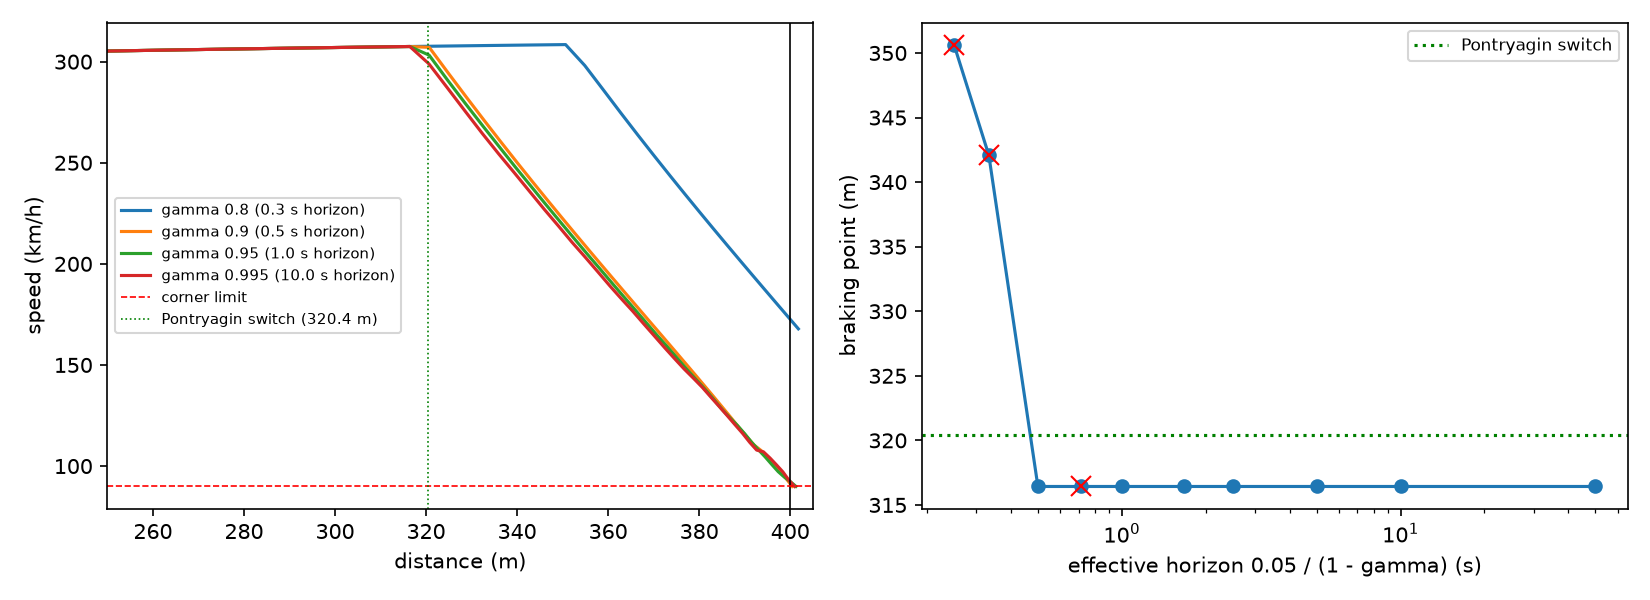
\includegraphics[width=\linewidth]{braking-gamma.png}
\caption{Left: speed against distance for four discount factors; the dotted line is
Pontryagin's switch point and the dashed line the corner's speed limit. Right: braking
point against the effective horizon; crosses mark crashes. Reproduced from the project's
findings (docs/findings/braking-gamma.png).}
\label{fig:braking}
\end{figure}

\paragraph{Reading} A crash forfeits all future progress, so its true cost is the
discounted value of everything after the corner. With a horizon of a few tenths of a
second that value is small, braking later gains more progress than the crash costs, and
the agent arrives at 144--168\,km/h. From $\gamma = 0.9$ on, every discounted optimum
brakes at 316.4\,m, one 50\,ms control step before Pontryagin's switch.
% src: docs/findings/braking-gamma.md ("Reading"); docs/STATUS.md (K3 row: "one 50 ms control
%      step before Pontryagin's switch point")

\paragraph{What this supports} Three things in the main text. First, the agent's objective
is not minimum time, and at short horizons the two optima disagree qualitatively; an
answer key built on lap time would charge such an agent with ``regret'' for doing exactly
what its objective asks. Second, at the $\gamma = 0.995$ the agent uses, the discounted and
minimum-time optima agree to within one control step on this problem, so the dense
progress reward produces racing behaviour without any lap-time term. Third, it is an
exact, independent check that a discounted optimum computed from the environment's reward
and crash penalty behaves as expected. The caveat is scale: this is a point mass in one
dimension, and the full-car counterpart is the TO-OCP itself.

\section{Supporting material: an audit with positive controls}
\label{app:snapping}
% src: docs/findings/snapping-audit.md (per-session table, reading, flagged list, skipped
%      sessions) and docs/findings/snapping-audit.png; docs/STATUS.md (P0 row) for the
%      archive size. Ranges below are min / median / max over the 85 session rows of the
%      table in docs/findings/snapping-audit.md, computed from that table.
% Lockbox note: this audit registers public F1 telemetry against real circuit geometry. It
% computes no agent return and no optimum on any circuit, which the plan allows.

This appendix is not used by any claim in the paper. It is included because it applies the
same discipline as the audit, a measurement validated with planted signals before it is
trusted, to the public data that a companion analysis of human drivers depends on, and
because its result fixes what that analysis can and cannot claim.

\paragraph{Question} Public Formula One timing data include car positions at about
3.7\,Hz. Do these positions carry each driver's racing line, or are they projected onto a
single track model? It has been stated informally that they carry no lateral line; we are
not aware of a quantitative audit.
% src: docs/plan/novelty-and-outputs.md (C6, FastF1 Discussion #116, OpenF1 docs)
\VERIFY{the claim of no prior quantitative audit rests on the plan's prior-art search}

\paragraph{Method} For every qualifying session, each flying lap's position samples are
compared with a cubic-spline curve through the pole lap. Two tests are run: the distance
of every sample from that curve, and whether a driver's \emph{signed} lateral offset is
consistent across their own laps at each 50\,m station (one-way ANOVA and the intraclass
correlation, ICC). Three positive controls check that the test can see a line if one is
there: pit-lane samples, which are metres from the racing line; whole laps shifted by known
offsets of 1--3\,m; and a planted 0.5\,m line for one driver.
% src: docs/findings/snapping-audit.md (opening paragraph)
The data are 85 sessions from 2023--26 with \num{8183} flying laps (OpenF1, CC BY-NC-SA
4.0; aggregate statistics only), drawn from an archive of 111 sessions whose 5,196 files
were all checksum-verified.
% src: docs/findings/snapping-audit.md (85 rows; laps column summed); docs/STATUS.md (P0 row)

\paragraph{Result} Every session looks the same. Samples sit a median 9.4--13.3\,cm from
the pole lap's curve (median over sessions 11.3\,cm), while pit-lane samples sit metres
away (95th percentile 7.9\,m or more in every session), so the feed can represent
off-line positions. Injected 2\,m offsets are recovered as 1.99--2.02\,m. Drivers'
offsets are not consistent: the median per-session driver ICC is 0.006 (range $-0.019$ to
$+0.068$). The planted 0.5\,m line, by contrast, reaches an ICC of 0.57--0.88 and is
detected at 88--100\% of stations (median 98\%).
% src: docs/findings/snapping-audit.md (columns "Median dist.", "Pit-lane p95", "Injected 2 m ->",
%      "Driver ICC", "Planted ICC", "Planted detected"; min / median / max over 85 rows)
A median of 3.5\% of stations (range 0--12.1\%) are individually significant at
$p < 0.01$. That is above the nominal 1\% but far below the planted line's rate; the source
report attributes the excess to centimetre-scale per-car artefacts such as antenna
position or latency, an explanation we have not tested.
% src: docs/findings/snapping-audit.md (column "Stations p<0.01"; "Flagged for follow-up" paragraph)
Twenty-two sessions are flagged as open items (more than 5\% of stations significant, or
driver offsets above 20\,cm at the 95th percentile, the latter only for the two
Silverstone sessions at about 40\,cm); one car with a coordinate stream about 3\,m off
everywhere was excluded and reported, and two sessions were skipped.
% src: docs/findings/snapping-audit.md ("Flagged for follow-up" list: 22 entries; "Excluded
%      cars": 2023 Jeddah car 21; "Skipped sessions": 2)

\begin{figure}[h]
\centering
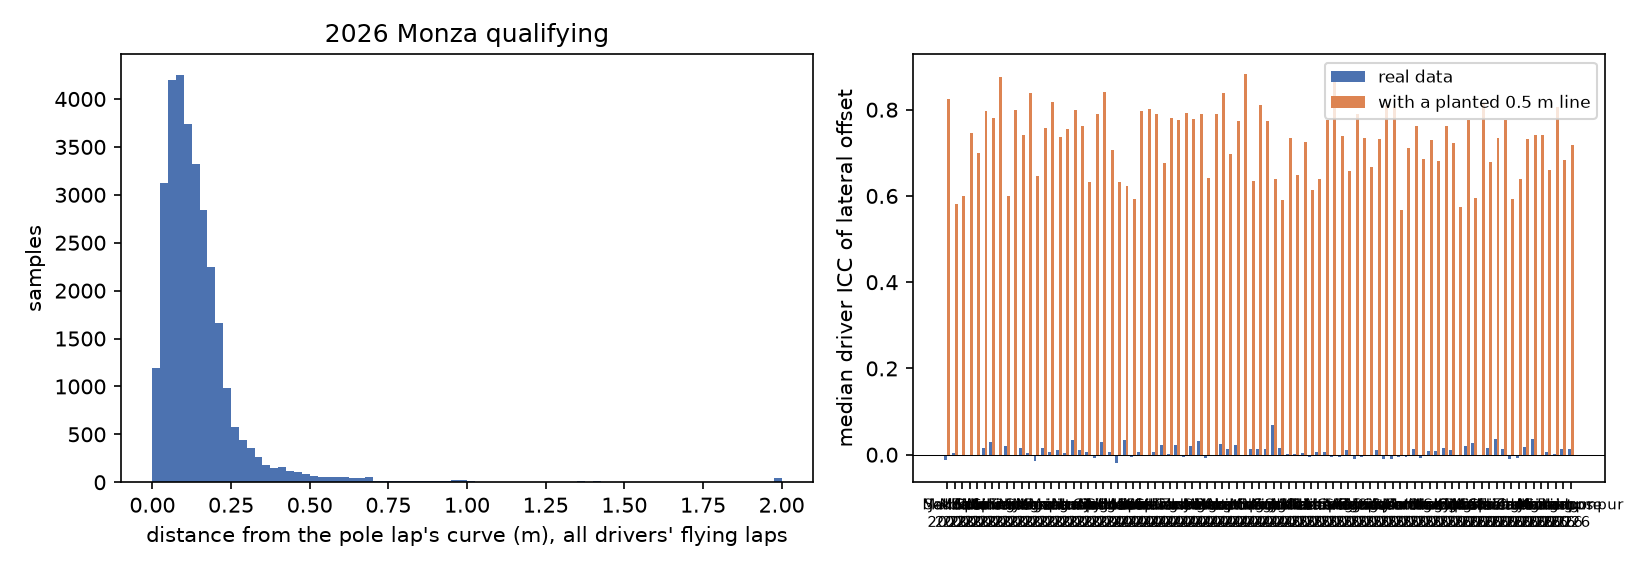
\includegraphics[width=\linewidth]{snapping-audit.png}
\caption{Left: distance of all drivers' flying-lap samples from the pole lap's curve in one
session. Right: median driver ICC of the signed lateral offset per session, for the real
data and with a planted 0.5\,m line. Reproduced from docs/findings/snapping-audit.png.}
\label{fig:snapping}
\end{figure}
\TODO{regenerate the right panel with legible session labels}

\paragraph{Consequence} The positions are projected onto one track model. Comparisons of
human drivers therefore use speed, throttle, brake and time as functions of distance,
never lateral lines. For this paper the lesson is methodological: a null result counts
only when the same pipeline demonstrably detects a planted signal of the size in question.


\end{document}
